\documentclass[11pt]{article}

\usepackage[margin=1in]{geometry}
\usepackage{amsmath,amssymb,amsthm,mathtools}
\usepackage{enumitem}
\usepackage{hyperref}
\usepackage{tikz}
\usetikzlibrary{arrows.meta,calc,decorations.markings,decorations.pathmorphing,
  patterns,positioning,shadings,shapes.geometric,fadings,3d,backgrounds,
  intersections,shapes.misc,bending}

\definecolor{formblue}{HTML}{1f4e79}
\definecolor{formteal}{HTML}{0f7077}
\definecolor{formsage}{HTML}{467b3a}
\definecolor{formgold}{HTML}{b88a14}
\definecolor{formrust}{HTML}{a8431d}
\definecolor{formplum}{HTML}{6b2e6e}
\definecolor{formmauve}{HTML}{84507a}
\definecolor{formslate}{HTML}{3a5168}
\definecolor{formivory}{HTML}{f6efe0}
\definecolor{formparch}{HTML}{ece2cb}
\definecolor{windingblue}{HTML}{1f3a8a}
\newcommand{\windingnote}[1]{%
\par\smallskip
\noindent\begin{minipage}{\linewidth}%
\color{windingblue}\small%
\textbf{\textit{Winding-form thread.}}\ \textit{#1}%
\end{minipage}\par\smallskip%
}
\definecolor{handink}{HTML}{1c2e63}
\definecolor{handsepia}{HTML}{8a5a2b}
\definecolor{handpaper}{HTML}{fbf6e9}
\tikzset{
  hand/.style={
    decorate,
    decoration={random steps, segment length=2.8mm, amplitude=0.32mm},
    line cap=round, line join=round,
    draw=handink, line width=0.55pt
  },
  handthick/.style={hand, line width=0.95pt},
  handthin/.style={hand, line width=0.4pt, opacity=0.85},
  handfill/.style={hand, fill=handink!8},
  handsepia/.style={hand, draw=handsepia},
  handnote/.style={font=\itshape\scriptsize, text=handink!85!black},
  handarrow/.style={draw=handink, -{Latex[length=2.2mm]}, line width=0.7pt, line cap=round},
  handpaper/.style={fill=handpaper, draw=handink!22, line width=0.4pt, rounded corners=2pt}
}
\newcommand{\handsketch}[1]{%
\par\smallskip\noindent
\begin{minipage}{\linewidth}\centering
\begin{tikzpicture}[scale=0.78, every node/.style={font=\scriptsize}, baseline]
\useasboundingbox (-3.6,-2.0) rectangle (3.6,2.0);
#1
\end{tikzpicture}
\end{minipage}\par\smallskip%
}

\tikzset{
  vector/.style={-{Latex[length=2.2mm]}, thick},
  formarrow/.style={-{Latex[length=2mm]}, thick, blue!65!black},
  region/.style={draw=blue!60!black, fill=blue!7, thick},
  hole/.style={draw=red!70!black, fill=white, thick},
  visualnode/.style={draw=black!55, rounded corners=2pt, align=center, inner sep=5pt, fill=black!3},
  tinyarrow/.style={-{Latex[length=1.7mm]}, thick},
  flowarrow/.style={-{Latex[length=3mm,width=2.4mm,bend]}, line width=0.7pt},
  ringfade/.style={inner color=#1!28, outer color=#1!2, draw=#1!50!black, thick},
  ringfade/.default=blue,
  artpanel/.style={draw=black!22, line width=0.5pt, rounded corners=2pt,
    inner color=formivory, outer color=formivory!85!black},
  doubleformarrow/.style={-{Latex[length=2.5mm]}, line width=0.9pt, draw=formplum},
  geodesic/.style={draw=formslate, thick, opacity=0.85},
  wavyform/.style={decorate, decoration={snake, amplitude=0.45mm, segment length=2.4mm}, thick}
}
\newcommand{\visualcaption}[1]{\par\smallskip{\small\emph{#1}}\par\medskip}

\allowdisplaybreaks
\setlist[enumerate]{leftmargin=*, itemsep=0.35em}

\newcommand{\C}{\mathbb{C}}
\newcommand{\R}{\mathbb{R}}
\newcommand{\CP}{\mathbb{CP}}
\newcommand{\Z}{\mathbb{Z}}
\newcommand{\dd}{\,d}
\newcommand{\ord}{\operatorname{ord}}
\newcommand{\Res}{\operatorname{Res}}
\newcommand{\divisor}{\operatorname{div}}
\newcommand{\degdiv}{\operatorname{deg}}
\newcommand{\id}{\operatorname{id}}
\newcommand{\im}{\operatorname{im}}
\newcommand{\eps}{\varepsilon}
\newenvironment{intentrequirements}{%
\paragraph{Intent and requirements.}
\begin{itemize}[leftmargin=*, itemsep=0.25em]
}{%
\end{itemize}
}

\title{Friendly Solutions to the Math 5312 / Math 7363 Final}
\author{}
\date{Spring 2026}

\begin{document}
\maketitle

\begin{center}
\emph{Study solutions for \texttt{Final\_Complex\_Analysis.pdf}. The exam instructions require handwritten submissions, so this file is intended as a reference for checking and learning the arguments.}
\end{center}

\paragraph{Conventions.}
All Riemann surfaces are connected unless otherwise stated. If $D=\sum n_p p$ is a divisor, then
\[
 L(D)=\{f\in \mathcal M(X):(f)+D\geq0\}\cup\{0\},
\]
and
\[
 I(D)=\{\omega\text{ meromorphic }1\text{-form}:(\omega)-D\geq0\}\cup\{0\}.
\]
We write $\ell(D)=\dim_\C L(D)$ and $i(D)=\dim_\C I(D)$.

\section*{Problem 1: Identity Theorem}

\begin{intentrequirements}
\item \textbf{Intent.} State and prove the theorem that holomorphic functions on a connected domain are determined by their values on any set with an accumulation point in the domain.
\item \textbf{Required outputs.} Give a precise statement for two holomorphic functions $f,g$, reduce the proof to $h=f-g$, prove that accumulating zeros force $h$ to vanish locally, and then use connectedness to conclude global vanishing.
\item \textbf{Required explanations.} Explain the isolated-zero argument from the Taylor expansion
\[
 h(z)=(z-a)^m u(z),\qquad u(a)\neq0,
\]
and explain why connectedness is needed to propagate local vanishing to the whole domain.
\item \textbf{Common pitfalls to avoid.} The accumulation point must lie inside the domain. Agreement on a set accumulating only at a boundary point is not enough.
\end{intentrequirements}

\windingnote{The Identity Theorem says holomorphic functions on a connected domain are determined by their germ at any interior accumulation point: there is no room for ``hidden'' multivaluedness in a single-valued holomorphic function. The winding form $\omega$ is the natural test case for the boundary of this principle: the locally-defined function $\arg(x+iy)$ on $\R^2\setminus\{0\}$ is \emph{multi-valued}, jumping by $2\pi$ along any loop encircling the origin. The Identity Theorem does \emph{not} prevent this: $\arg$ is not a single global holomorphic function, but a section of a non-trivial covering. So the winding form is what survives in cohomology when ``$\arg$ should have been single-valued but isn't.'' This sets the stage for analytic continuation in Problem~2 (where $\log z$ exhibits exactly the same monodromy).}

\handsketch{%
\fill[handpaper] (-3.4,-1.9) rectangle (3.4,1.9);
\draw[hand] (-3.4,-1.9) rectangle (3.4,1.9);
% Punctured plane
\fill[handink] (0,0) circle (0.05);
\node[handnote] at (-0.18,-0.15) {$0$};
% Spiral showing arg increasing each turn
\draw[draw=handink, line width=0.55pt, domain=0:8, samples=120, smooth, variable=\t]
  plot ({(0.18+0.06*\t)*cos(\t r)},{(0.18+0.06*\t)*sin(\t r)});
% Arrows along spiral
\draw[handarrow] ({(0.18+0.06*2.0)*cos(2.0 r)},{(0.18+0.06*2.0)*sin(2.0 r)}) --
                ({(0.18+0.06*2.2)*cos(2.2 r)},{(0.18+0.06*2.2)*sin(2.2 r)});
% Notation
\node[handnote] at (-2.4,1.55) {$\arg(x+iy)$};
\node[handnote] at (-2.4,1.15) {multi-valued};
\node[handnote] at (2.4,1.55) {$+2\pi$ per loop};
\node[handnote] at (2.4,-1.55) {Identity Thm};
\node[handnote] at (2.4,-1.85) {does not stop this};
}

\textbf{Theorem.}
Let $\Omega\subset\C$ be a connected domain, and let $f,g$ be holomorphic on $\Omega$.
If the set
\[
 \{z\in\Omega:f(z)=g(z)\}
\]
has an accumulation point in $\Omega$, then $f=g$ on all of $\Omega$.
Equivalently, if a holomorphic function $h$ on a connected domain has zeros accumulating at a point of the domain, then $h\equiv0$.

\textbf{Proof.}
Apply the equivalent form to
\[
 h=f-g.
\]
Let $a\in\Omega$ be an accumulation point of zeros of $h$.
The Taylor expansion of $h$ at $a$ has the form
\[
 h(z)=\sum_{n=0}^{\infty}c_n(z-a)^n.
\]
If not all $c_n$ were zero, let $m$ be the first index with $c_m\neq0$. Then
\[
 h(z)=(z-a)^m u(z),
 \qquad u(a)=c_m\neq0.
\]
After shrinking the disk around $a$, $u$ is nonzero, so $a$ would be an isolated zero of $h$. This contradicts the assumed accumulation of zeros at $a$. Hence all Taylor coefficients vanish, and $h$ vanishes on some disk around $a$.

Now let
\[
 S=\{p\in\Omega:h\text{ vanishes on a neighborhood of }p\}.
\]
The set $S$ is nonempty by the previous paragraph. It is open by definition. It is also closed in $\Omega$: if $p_j\in S$ and $p_j\to p$, then $h(p_j)=0$, so $p$ is an accumulation point of zeros unless eventually $p_j=p$; in either case the same Taylor-series argument shows that $h$ vanishes near $p$.
Since $\Omega$ is connected, $S=\Omega$. Thus $h\equiv0$, so $f=g$.

\begin{center}
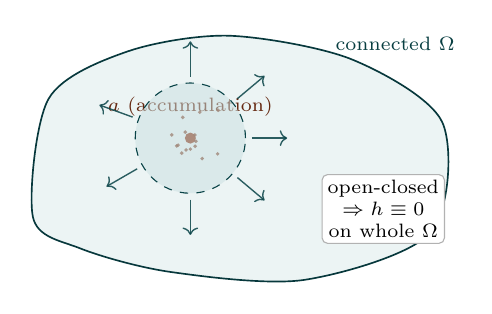
\begin{tikzpicture}[scale=1.0, every node/.style={font=\scriptsize}]
% Connected domain
\filldraw[draw=formteal!50!black, fill=formteal!8, line width=0.6pt]
  plot[smooth cycle] coordinates {(-2.6,-0.65) (-2.4,0.85) (-1.4,1.45) (-0.1,1.65) (1.45,1.35) (2.6,0.55) (2.45,-0.85) (0.85,-1.45) (-0.85,-1.35) (-2.0,-1.05)};
% Accumulation point and nearby zeros
\coordinate (A) at (-0.6,0.35);
\fill[formrust!85!black] (A) circle (0.07);
\node[formrust!60!black, font=\scriptsize, above] at (-0.6,0.5) {$a$ (accumulation)};
\foreach \r/\sx/\sy in {0.5/45/20, 0.4/-30/-15, 0.35/70/60, 0.3/-60/-35, 0.28/110/40,
                       0.24/170/55, 0.22/-120/30, 0.2/210/60, 0.18/-150/15, 0.16/250/40,
                       0.14/-90/65, 0.12/300/25, 0.10/130/15, 0.08/-30/40, 0.07/35/-10}{
  \pgfmathsetmacro\xx{-0.6+\r*cos(\sx)}
  \pgfmathsetmacro\yy{0.35+\r*sin(\sx)}
  \fill[formrust!70!black, opacity=0.8] (\xx,\yy) circle (0.025);
}
% Propagation: filled vanishing region
\filldraw[draw=formteal!60!black, fill=formteal!22, fill opacity=0.5, line width=0.4pt, dashed] (A) circle (0.7);
% Arrows showing propagation
\foreach \th in {0,40,90,160,210,270,320}{
  \draw[->, formteal!60!black, line width=0.5pt, opacity=0.85] ($(A)+(\th:0.78)$) -- ++(\th:0.45);
}
\node[font=\scriptsize, fill=white, rounded corners=2pt, inner sep=2pt, draw=black!30, align=center]
  at (1.85,-0.55) {open-closed\\$\Rightarrow h\equiv0$\\on whole $\Omega$};
\node[font=\scriptsize, formteal!55!black] at (2.0,1.55) {connected $\Omega$};
\end{tikzpicture}
\visualcaption{Accumulating zeros at one interior point force $h$ to vanish on an open neighborhood there; the set where $h$ vanishes locally is both open and closed in the connected domain, hence the whole domain.}
\end{center}

\section*{Problem 2: Analytic Continuation}

\begin{intentrequirements}
\item \textbf{Intent.} Use the Identity Theorem to extend the real Maclaurin series identity for $\sin x$ to the entire complex plane.
\item \textbf{Required outputs.} Show that the power series defining $g$ has infinite radius of convergence, observe that $f(z)=\sin z$ and $g(z)$ are entire, verify equality on the real axis, and conclude equality on $\C$.
\item \textbf{Required explanations.} Explain why the real axis supplies a set of agreement points with an accumulation point in the connected complex domain $\C$.
\item \textbf{Common pitfalls to avoid.} Do not try to reprove complex convergence pointwise after the identity theorem step. Once both functions are entire and agree on a set with a limit point, the conclusion is global.
\end{intentrequirements}

\windingnote{The contrast between $\sin z$ and $\log z$ illuminates why the winding form matters. The function $\sin z$ extends from $\R$ to $\C$ uniquely and \emph{single-valued} because both $\sin z$ and its Maclaurin series are \emph{entire} (holomorphic on all of $\C$), so the Identity Theorem closes the deal. But $\log z$ has no holomorphic extension to all of $\C\setminus\{0\}$: any local branch differs from another by an integer multiple of $2\pi i$, and traversing a loop around the origin shifts the value by $2\pi i$. The differential $d\log z=dz/z$ is single-valued and \emph{is} the complexification of the winding form $\omega$ via $dz/z=\tfrac{x\,dx+y\,dy}{x^2+y^2}+i\omega$. So while functions can sometimes be analytically continued, their \emph{integrals} along loops detect winding via the winding form, and that detection is exactly what the multivaluedness of $\log$ records.}

\handsketch{%
\fill[handpaper] (-3.4,-1.9) rectangle (3.4,1.9);
\draw[hand] (-3.4,-1.9) rectangle (3.4,1.9);
% Left: sin z extends to C
\begin{scope}[xshift=-1.85cm]
  \draw[handthick] (-1.0,-1.0) rectangle (1.0,1.0);
  \draw[draw=handink, line width=0.5pt] (-0.85,0) -- (0.85,0);
  \draw[draw=handink, line width=0.4pt, samples=60, smooth, variable=\x, domain=-0.85:0.85]
    plot (\x, {0.35*sin(180*\x*1.4)});
  \node[handnote] at (0,1.25) {$\sin z$};
  \node[handnote] at (0,-1.25) {entire $\Rightarrow$ unique};
\end{scope}
% Right: log z with branch cut
\begin{scope}[xshift=1.85cm]
  \draw[handthick] (-1.0,-1.0) rectangle (1.0,1.0);
  \fill[handink] (0,0) circle (0.06);
  \draw[draw=handink, dashed, line width=0.5pt] (-1.0,0) -- (-0.07,0);
  % Loop around 0
  \draw[draw=handink, line width=0.6pt, -{Latex[length=1.8mm]}] (35:0.55) arc (35:325:0.55);
  \node[handnote] at (0,1.25) {$\log z$};
  \node[handnote] at (0,-1.25) {$+2\pi i$ per turn};
\end{scope}
\node[handnote] at (0,1.7) {$d\log z=dz/z=(\text{rad})+i\,\omega$};
}

Let
\[
 f(z)=\sin z,\qquad
 g(z)=\sum_{n=0}^{\infty}(-1)^n\frac{z^{2n+1}}{(2n+1)!}.
\]
The series defining $g$ has infinite radius of convergence, so $g$ is entire. The function $f$ is also entire.

For real $x$, the usual real Maclaurin theorem for sine gives
\[
 \sin x=\sum_{n=0}^{\infty}(-1)^n\frac{x^{2n+1}}{(2n+1)!}.
\]
Therefore
\[
 f(x)=g(x)
\]
for every real $x$. The real axis has accumulation points in $\C$, for example $0$. Hence the holomorphic function $f-g$ has zeros with an accumulation point in the connected domain $\C$.
By the Identity Theorem,
\[
 f(z)=g(z)
\]
for every $z\in\C$.

\begin{center}
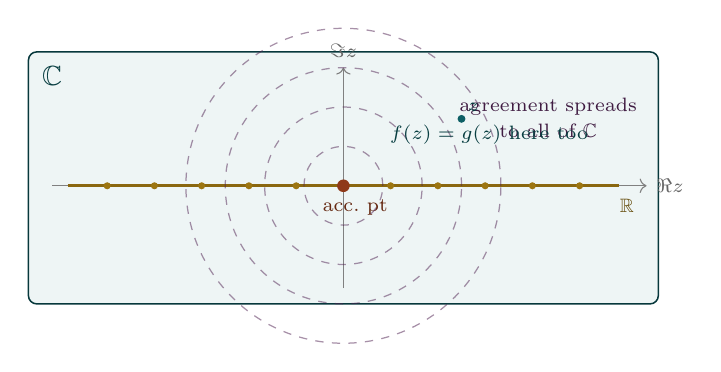
\begin{tikzpicture}[scale=1.0, every node/.style={font=\scriptsize}]
% Complex plane
\filldraw[draw=formteal!50!black, fill=formteal!7, line width=0.55pt, rounded corners=3pt]
  (-4.0,-1.5) rectangle (4.0,1.7);
\node[formteal!55!black, font=\bfseries] at (-3.7,1.4) {$\C$};
% Axes
\draw[->, black!50, line width=0.4pt] (-3.7,0) -- (3.85,0) node[right, black!60] {$\Re z$};
\draw[->, black!50, line width=0.4pt] (0,-1.3) -- (0,1.5) node[above, black!60] {$\Im z$};
% Real axis highlighted: agreement set
\draw[formgold!75!black, line width=1.2pt] (-3.5,0) -- (3.5,0);
\foreach \xx in {-3.0,-2.4,-1.8,-1.2,-0.6,0.6,1.2,1.8,2.4,3.0}{
  \fill[formgold!85!black] (\xx,0) circle (0.045);
}
\node[formgold!55!black, font=\scriptsize, below] at (3.6,-0.05) {$\R$};
% Accumulation point
\fill[formrust!85!black] (0,0) circle (0.08);
\node[formrust!60!black, font=\scriptsize] at (0.15,-0.27) {acc.\ pt};
% Propagating wavefront — the Identity Theorem spreads agreement
\foreach \rr/\op in {0.5/30, 1.0/22, 1.5/14, 2.0/8}{
  \draw[dashed, formplum!75!black, line width=0.45pt, opacity=0.5] (0,0) circle (\rr);
}
\node[formplum!60!black, font=\scriptsize] at (2.6,1.0) {agreement spreads};
\node[formplum!60!black, font=\scriptsize] at (2.6,0.7) {to all of $\C$};
% Sample point off real axis where equality is now forced
\fill[formteal!85!black] (1.5,0.85) circle (0.05);
\node[formteal!55!black, font=\scriptsize] at (1.65,1.0) {$z$};
\node[formteal!55!black, font=\scriptsize, align=left] at (1.85,0.65) {$f(z)=g(z)$ here too};
\end{tikzpicture}
\visualcaption{Real-axis agreement is a one-dimensional dataset with accumulation in two-dimensional $\C$. The Identity Theorem promotes it to global agreement: a single line of equality determines the entire entire function.}
\end{center}

\section*{Problem 3: Open Mapping Theorem}

\begin{intentrequirements}
\item \textbf{Intent.} Prove that a nonconstant holomorphic function maps open sets to open sets.
\item \textbf{Required outputs.} State the theorem precisely, reduce to showing a neighborhood of $f(a)$ lies in the image of a small disk around $a$, use the finite-order local factorization of $f(z)-f(a)$, and finish with Rouche's theorem.
\item \textbf{Required explanations.} Explain why the minimum of $|f(z)-f(a)|$ on a sufficiently small boundary circle is positive, and why Rouche's theorem guarantees a solution to $f(z)=w$ for $w$ near $f(a)$.
\item \textbf{Common pitfalls to avoid.} The theorem requires nonconstancy. Constant holomorphic maps are not open as maps into $\C$.
\end{intentrequirements}

\windingnote{The Rouch\'e step in the proof is a direct application of the winding form. Specifically: the argument principle states $\frac{1}{2\pi i}\oint_{|z-a|=r}\frac{f'(z)}{f(z)-w_0}\,dz=\#\{z\in B_r(a):f(z)=w_0\}$ counted with multiplicity. The integrand $\frac{f'(z)\,dz}{f(z)-w_0}$ is the pull-back of the winding form $dz/z$ by $f-w_0$, and the integral computes the winding number of $f-w_0$ around $0$. When $|w-w_0|<\delta$, this winding number stays the same for $f-w$, so $f-w$ has the same number of zeros in $B_r(a)$ --- i.e.\ $w$ is in the image. Open Mapping is, at its core, the statement that winding numbers do not decrease under small perturbations.}

\handsketch{%
\fill[handpaper] (-3.4,-1.9) rectangle (3.4,1.9);
\draw[hand] (-3.4,-1.9) rectangle (3.4,1.9);
% Source disk
\begin{scope}[xshift=-1.85cm]
  \draw[handthick] (0,0) circle (1.0);
  \fill[handink] (0,0) circle (0.04);
  \node[handnote] at (0.15,-0.1) {$a$};
  \node[handnote] at (0,1.3) {$|z-a|=r$};
\end{scope}
% Map arrow
\draw[draw=handink, line width=0.8pt, -{Latex[length=2.5mm]}] (-0.7,0) -- (0.5,0);
\node[handnote] at (-0.1,0.3) {$f-w$};
% Target with winding curve around 0
\begin{scope}[xshift=1.85cm]
  \draw[handthick] (0,0) circle (1.1);
  \fill[handink] (0,0) circle (0.05);
  \node[handnote] at (0.18,-0.2) {$0$};
  % Curve winding around 0
  \draw[draw=handink, line width=0.6pt, smooth, samples=80, variable=\t, domain=0:360]
    plot ({(0.55+0.18*sin(2*\t))*cos(\t)},{(0.55+0.18*sin(2*\t))*sin(\t)});
  % small w near w_0
  \fill[handink] (-0.2,0.18) circle (0.03);
  \node[handnote] at (-0.05,0.3) {$w$};
  \node[handnote] at (0,-1.4) {winding $=\#$ roots};
\end{scope}
\node[handnote] at (0,1.75) {argument principle};
}

\textbf{Theorem.}
Let $\Omega\subset\C$ be a domain and let $f:\Omega\to\C$ be holomorphic and nonconstant. Then $f$ is an open map: for every open set $U\subset\Omega$, the image $f(U)$ is open in $\C$.

\textbf{Proof.}
It is enough to prove that for every $a\in\Omega$ and every sufficiently small disk around $a$, the image contains a disk around $f(a)$.
Set
\[
 w_0=f(a).
\]
Since $f$ is not locally constant, the zero of $f(z)-w_0$ at $a$ has some finite order $m\geq1$. Thus
\[
 f(z)-w_0=(z-a)^m u(z),
\]
where $u$ is holomorphic and $u(a)\neq0$.

Choose $r>0$ so small that the closed disk $\overline{B_r(a)}$ lies in $\Omega$ and $f(z)\neq w_0$ on the circle $|z-a|=r$. Let
\[
 \delta=\min_{|z-a|=r}|f(z)-w_0|>0.
\]
If $|w-w_0|<\delta$, then on $|z-a|=r$ we have
\[
 |w-w_0|<|f(z)-w_0|.
\]
By Rouche's theorem, the functions $f(z)-w_0$ and $f(z)-w$ have the same number of zeros in $B_r(a)$, counted with multiplicity. Since $f(z)-w_0$ has at least one zero there, so does $f(z)-w$.
Thus every $w$ with $|w-w_0|<\delta$ belongs to $f(B_r(a))$.

So $f(U)$ contains a neighborhood of each of its points, and hence $f(U)$ is open.

\begin{center}
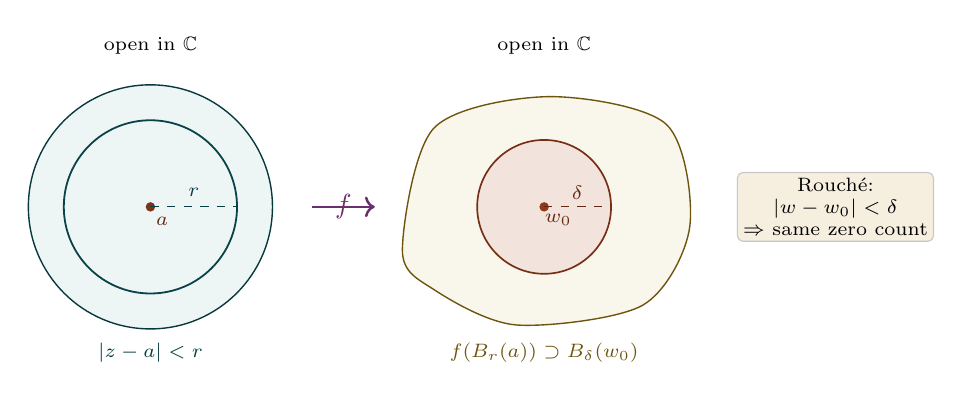
\begin{tikzpicture}[scale=1.0, every node/.style={font=\scriptsize}]
% Source disk
\begin{scope}
  \filldraw[draw=formteal!50!black, fill=formteal!7, line width=0.5pt] (0,0) circle (1.55);
  \draw[draw=formteal!60!black, line width=0.65pt] (0,0) circle (1.1);
  \fill[formrust!75!black] (0,0) circle (0.06);
  \node[formrust!60!black, font=\scriptsize] at (0.15,-0.18) {$a$};
  \draw[dashed, formteal!55!black, line width=0.4pt] (0,0) -- (1.1,0);
  \node[formteal!55!black, font=\scriptsize] at (0.55,0.18) {$r$};
  \node[formteal!55!black, font=\scriptsize] at (0,-1.85) {$|z-a|<r$};
\end{scope}
% Arrow with f
\node[formplum, font=\bfseries] at (2.45,0) {$f$};
\draw[->, formplum, line width=0.9pt] (2.05,0) -- (2.85,0);
% Image: disk around f(a)
\begin{scope}[xshift=5.0cm]
  \filldraw[draw=formgold!60!black, fill=formgold!8, line width=0.5pt]
    plot[smooth cycle] coordinates {(-1.8,-0.55) (-1.4,1.0) (0.05,1.4) (1.55,1.05) (1.85,-0.25) (1.25,-1.25) (-0.35,-1.5) (-1.4,-1.05)};
  % Inner disk B_delta(w_0)
  \filldraw[draw=formrust!70!black, fill=formrust!15, line width=0.6pt] (0,0) circle (0.85);
  \fill[formrust!85!black] (0,0) circle (0.06);
  \node[formrust!60!black, font=\scriptsize] at (0.18,-0.16) {$w_0$};
  \draw[dashed, formrust!60!black, line width=0.4pt] (0,0) -- (0.85,0);
  \node[formrust!60!black, font=\scriptsize] at (0.42,0.18) {$\delta$};
  \node[formgold!60!black, font=\scriptsize] at (0,-1.85) {$f(B_r(a))\supset B_\delta(w_0)$};
\end{scope}
% Captions
\node[font=\scriptsize, align=center] at (0,2.05) {open in $\C$};
\node[font=\scriptsize, align=center] at (5.0,2.05) {open in $\C$};
\node[font=\scriptsize, align=center, fill=formivory, rounded corners=2pt, inner sep=2pt, draw=black!22]
  at (8.7,0) {Rouch\'e: \\$|w-w_0|<\delta$\\$\Rightarrow$ same zero count};
\end{tikzpicture}
\visualcaption{The proof shows that the image of the small disk $B_r(a)$ contains a whole disk $B_\delta(w_0)$ around the image point. The key estimate $\delta=\min_{|z-a|=r}|f(z)-w_0|$ is positive because $f$ is nonconstant.}
\end{center}

\section*{Problem 4: Related Example for the Open Mapping Theorem}

\begin{intentrequirements}
\item \textbf{Intent.} Apply the Open Mapping Theorem to a concrete holomorphic map and domain.
\item \textbf{Required outputs.} Identify $B_1(1)$ as an open connected subset of $\C$, note that $f(z)=z^2$ is holomorphic and nonconstant there, and conclude that $f(B_1(1))$ is open.
\item \textbf{Required explanations.} Optionally explain the stronger local-biholomorphism fact: $f'(z)=2z$ does not vanish inside $B_1(1)$ because $0$ lies on the boundary, not in the disk.
\item \textbf{Common pitfalls to avoid.} Do not confuse the image's geometric shape with the question being asked. The problem only asks for openness, not an explicit description of the image.
\end{intentrequirements}

Let
\[
 f(z)=z^2,\qquad B_1(1)=\{z\in\C:|z-1|<1\}.
\]
The disk $B_1(1)$ is open and connected. The function $f(z)=z^2$ is holomorphic and nonconstant on this disk. Therefore, by the Open Mapping Theorem,
\[
 f(B_1(1))
\]
is an open subset of $\C$.

One can also see this locally. The only critical point of $z^2$ is $0$, and $0$ is not in $B_1(1)$ because $|0-1|=1$. Hence $f'(z)=2z\neq0$ throughout $B_1(1)$, so $f$ is locally biholomorphic at every point of the disk. Therefore every image point has a small open neighborhood contained in the image.

\windingnote{The map $z\mapsto z^2$ on a circle around $0$ \emph{doubles} winding numbers: the image of $|z|=r$ wraps the origin twice. If $B_1(1)$ contained the critical point $0$, the local model at $0$ would be $z\mapsto z^2$, and a loop around the critical point would map to a loop with winding $2$ around the image; the local degree there is $2$. Excluding $0$ from $B_1(1)$ keeps the winding at $1$ on every infinitesimal loop, which is what ``locally biholomorphic'' really says: the winding-form pull-back $f^*(dz/z)=2z\,dz/z^2=2\,dz/z$ has residue $2$ at $z=0$ but is regular elsewhere. The pull-back winding $2$ at a critical point is exactly the ramification index that returns in Problem~5.}

\handsketch{%
\fill[handpaper] (-3.4,-1.9) rectangle (3.4,1.9);
\draw[hand] (-3.4,-1.9) rectangle (3.4,1.9);
% Source loop (one wind)
\begin{scope}[xshift=-1.85cm]
  \draw[handthick] (0,0) circle (0.95);
  \draw[draw=handink, line width=0.55pt, -{Latex[length=1.7mm]}] (40:0.95) arc (40:160:0.95);
  \fill[handink] (0,0) circle (0.04);
  \node[handnote] at (0,1.2) {$|z|=r$};
  \node[handnote] at (0,-1.25) {winding $=1$};
\end{scope}
% Map arrow
\draw[draw=handink, line width=0.8pt, -{Latex[length=2.5mm]}] (-0.65,0) -- (0.55,0);
\node[handnote] at (0,0.3) {$z\mapsto z^2$};
% Target: loop traversed twice
\begin{scope}[xshift=1.85cm]
  \draw[draw=handink, line width=0.6pt, smooth, samples=100, variable=\t, domain=0:720]
    plot ({(0.9+0.05*sin(4*\t))*cos(\t)},{(0.9+0.05*sin(4*\t))*sin(\t)});
  \fill[handink] (0,0) circle (0.04);
  \node[handnote] at (0,1.2) {$|w|=r^{2}$};
  \node[handnote] at (0,-1.25) {winding $=2$};
\end{scope}
\node[handnote] at (0,1.75) {$z\mapsto z^2$ doubles the winding};
}

\begin{center}
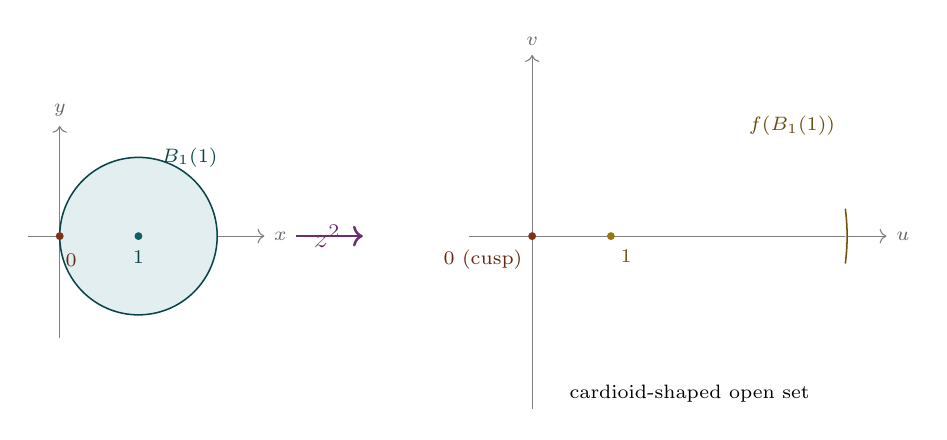
\begin{tikzpicture}[scale=1.0, every node/.style={font=\scriptsize}]
% Source: B_1(1)
\begin{scope}
  \draw[->, black!50, line width=0.4pt] (-0.4,0) -- (2.6,0) node[right, black!60] {$x$};
  \draw[->, black!50, line width=0.4pt] (0,-1.3) -- (0,1.4) node[above, black!60] {$y$};
  \filldraw[draw=formteal!60!black, fill=formteal!12, line width=0.55pt] (1,0) circle (1.0);
  \fill[formrust!75!black] (0,0) circle (0.05);
  \node[formrust!60!black, font=\scriptsize, below right] at (-0.05,-0.1) {$0$};
  \fill[formteal!85!black] (1,0) circle (0.05);
  \node[formteal!60!black, font=\scriptsize, below] at (1.0,-0.07) {$1$};
  \node[formteal!60!black, font=\scriptsize] at (1.65,1.0) {$B_1(1)$};
\end{scope}
% Arrow
\node[formplum, font=\bfseries] at (3.4,0) {$z^2$};
\draw[->, formplum, line width=0.9pt] (3.0,0) -- (3.85,0);
% Image (cardioid-like region; image of B_1(1) under z^2 is the cardioid r=2(1+cos theta))
\begin{scope}[xshift=6.0cm]
  \draw[->, black!50, line width=0.4pt] (-0.8,0) -- (4.5,0) node[right, black!60] {$u$};
  \draw[->, black!50, line width=0.4pt] (0,-2.2) -- (0,2.3) node[above, black!60] {$v$};
  % cardioid: in polar (rho, phi), rho = 2 + 2 cos phi, but for z^2 of disk |z-1|=1 (where z = 1 + e^{it}),
  % z^2 = 1 + 2e^{it} + e^{2it}.
  \draw[draw=formgold!60!black, fill=formgold!12, line width=0.55pt, samples=120, smooth, variable=\t]
    plot ({1 + 2*cos(\t) + cos(2*\t)},{2*sin(\t) + sin(2*\t)});
  \fill[formrust!75!black] (0,0) circle (0.05);
  \node[formrust!60!black, font=\scriptsize, below left] at (0,-0.05) {$0$ (cusp)};
  \fill[formgold!85!black] (1,0) circle (0.05);
  \node[formgold!60!black, font=\scriptsize, below right] at (1,-0.05) {$1$};
  \node[formgold!55!black, font=\scriptsize] at (3.3,1.4) {$f(B_1(1))$};
  \node[font=\scriptsize] at (2,-2.0) {cardioid-shaped open set};
\end{scope}
\end{tikzpicture}
\visualcaption{The disk $B_1(1)$ excludes $0$ from its interior; $z^2$ is locally biholomorphic on it, and the image is the open cardioid $\{|w|<2+2\Re\sqrt{w}\}$. The Open Mapping Theorem guarantees openness without identifying the boundary shape.}
\end{center}

\section*{Problem 5: Holomorphic Maps Between Compact Riemann Surfaces}

\begin{intentrequirements}
\item \textbf{Intent.} State and prove the main structural result for nonconstant holomorphic maps between compact Riemann surfaces: such maps are finite branched coverings with a well-defined degree.
\item \textbf{Required outputs.} Prove surjectivity, finiteness of fibers, finiteness of ramification points, the covering-map property away from branch values, and the fiber-degree formula
\[
 \sum_{x\in f^{-1}(y)}e_x(f)=\deg f.
\]
\item \textbf{Required explanations.} Use compactness plus the Open Mapping Theorem for surjectivity, the Identity Theorem for discreteness of fibers, and the local normal form $w=z^{e_x}$ for ramification.
\item \textbf{Common pitfalls to avoid.} The ordinary number of points in a fiber may drop over branch values. The degree counts points with ramification multiplicity.
\end{intentrequirements}

\windingnote{The ramification index $e_x(f)$ at a point $x$ is the \emph{local winding} of $f$. In a local coordinate $z$ at $x$ and $w$ at $f(x)$, the map looks like $w=z^{e_x}$; a small positively oriented loop $|z|=\eps$ pushes forward to $|w|=\eps^{e_x}$ traversed $e_x$ times. In winding-form language, $f^*(dw/w)=e_x\cdot dz/z+\text{(holomorphic)}$, so the pull-back winding form has residue $e_x$ at $x$. The fiber-degree formula $\sum_{x\in f^{-1}(y)}e_x(f)=\deg f$ then reads: the total local winding over a fiber equals the degree of $f$, i.e.\ the global winding count of $f$ around any regular value. This is the residue theorem for the pull-back of $dw/w$.}

\handsketch{%
\fill[handpaper] (-3.4,-1.9) rectangle (3.4,1.9);
\draw[hand] (-3.4,-1.9) rectangle (3.4,1.9);
% Source neighborhood (one loop)
\begin{scope}[xshift=-1.85cm]
  \draw[handthick] (0,0) circle (0.85);
  \fill[handink] (0,0) circle (0.05);
  \node[handnote] at (0.16,-0.18) {$x$};
  \draw[draw=handink, line width=0.55pt, -{Latex[length=1.7mm]}] (50:0.85) arc (50:140:0.85);
  \node[handnote] at (0,1.1) {coord $z$};
\end{scope}
% Arrow
\draw[draw=handink, line width=0.8pt, -{Latex[length=2.5mm]}] (-0.7,0) -- (0.45,0);
\node[handnote] at (-0.1,0.3) {$w=z^{e_x}$};
% Target: e_x-fold winding
\begin{scope}[xshift=1.85cm]
  \draw[draw=handink, line width=0.6pt, smooth, samples=120, variable=\t, domain=0:1080]
    plot ({(0.85+0.03*sin(8*\t))*cos(\t)},{(0.85+0.03*sin(8*\t))*sin(\t)});
  \fill[handink] (0,0) circle (0.05);
  \node[handnote] at (0.16,-0.18) {$f(x)$};
  \node[handnote] at (0,1.1) {coord $w$};
\end{scope}
\node[handnote] at (-1.85,-1.4) {winding $1$};
\node[handnote] at (1.85,-1.4) {winding $e_x=3$ (drawn)};
\node[handnote] at (0,-1.85) {$f^*(dw/w)=e_x\,dz/z+\text{(reg.)}$};
}

\textbf{Proposition.}
Let
\[
 f:X\to Y
\]
be a nonconstant holomorphic map between compact Riemann surfaces. Then:
\begin{enumerate}
\item $f(X)=Y$.
\item Each fiber $f^{-1}(y)$ is finite.
\item The set of ramification points is finite.
\item Away from the branch values, $f$ is a covering map.
\item There is an integer $n=\deg f$ such that for every $y\in Y$,
\[
 \sum_{x\in f^{-1}(y)}e_x(f)=n,
\]
where $e_x(f)$ is the ramification index of $f$ at $x$.
\end{enumerate}

\textbf{Proof.}
First, $f(X)$ is compact because $X$ is compact. Since $Y$ is Hausdorff, $f(X)$ is closed in $Y$. By the Open Mapping Theorem, $f(X)$ is also open because $f$ is nonconstant. The image is nonempty, open, and closed in the connected surface $Y$, so
\[
 f(X)=Y.
\]

Fix $y\in Y$. The fiber $f^{-1}(y)$ is closed in $X$, hence compact. It is also discrete. Indeed, if points of $f^{-1}(y)$ accumulated at $x\in X$, then in local coordinates the holomorphic function $f-y$ would have zeros accumulating at $x$, so the Identity Theorem would force $f$ to be locally constant and then globally constant. That contradicts the hypothesis. A compact discrete set is finite, so each fiber is finite.

In local coordinates near $x\in X$ and $f(x)\in Y$, the map has the form
\[
 w=f(z).
\]
After translating coordinates, this can be written as
\[
 w=z^{e_x}u(z),
\qquad u(0)\neq0,
\]
and after changing the target coordinate one can write locally
\[
 w=z^{e_x}.
\]
The point $x$ is ramified exactly when $e_x>1$, equivalently when the local derivative vanishes. The zeros of a nonzero holomorphic derivative are isolated. Since $X$ is compact, there can be only finitely many ramification points.

Let $R\subset X$ be the finite set of ramification points and let
\[
 B=f(R)\subset Y
\]
be the finite set of branch values. If $y\in Y\setminus B$, every point of $f^{-1}(y)$ is unramified. Around each $x\in f^{-1}(y)$, the map is a biholomorphism onto a small disk around $y$. Choosing the disk small enough and using the finiteness of the fiber, the inverse image of that disk is a disjoint union of such neighborhoods, each mapped biholomorphically onto the disk. Hence
\[
 f:X\setminus f^{-1}(B)\to Y\setminus B
\]
is a covering map.

On the connected surface $Y\setminus B$, the number of points in an unramified fiber is locally constant, hence constant. Call this number $n=\deg f$.
For a branch value $y_0$, choose a small disk $V$ around $y_0$ containing no other branch values. If
\[
 f^{-1}(y_0)=\{x_1,\dots,x_r\},
\]
then locally near $x_j$ the map is $z\mapsto z^{e_{x_j}}$. For $y\in V\setminus\{y_0\}$, this local model contributes exactly $e_{x_j}$ distinct preimages near $x_j$. Therefore
\[
 n=\sum_{j=1}^r e_{x_j}(f).
\]
This proves the fiber-degree formula for every fiber.

\begin{center}
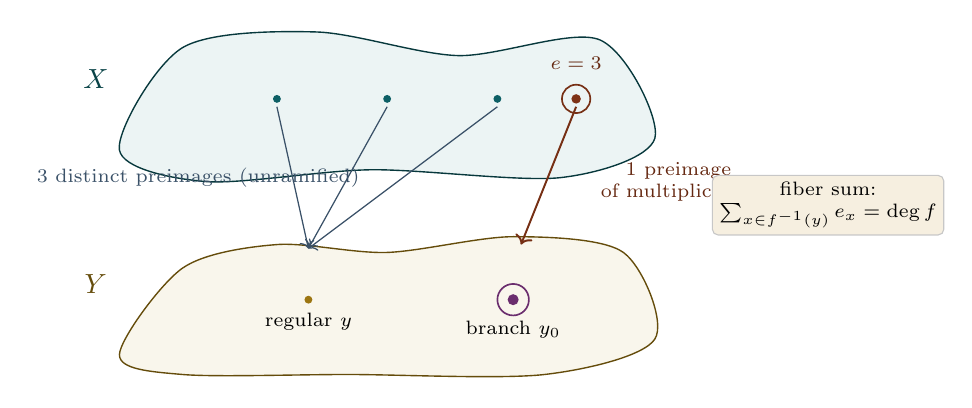
\begin{tikzpicture}[scale=1.0, every node/.style={font=\scriptsize}]
% Top: source with sheets
\begin{scope}[yshift=2.0cm]
  \filldraw[draw=formteal!50!black, fill=formteal!8, line width=0.5pt]
    plot[smooth cycle] coordinates {(-3.4,-0.6) (-2.6,0.7) (-0.9,0.9) (0.9,0.6) (2.7,0.8) (3.4,-0.45) (2.2,-0.95) (-0.2,-0.85) (-2.3,-1.0)};
  \node[formteal!60!black, font=\bfseries] at (-3.7,0.3) {$X$};
  % Three points: two unramified, one ramified
  \foreach \x in {-1.4,0.0,1.4}{
    \fill[formteal!85!black] (\x,0.05) circle (0.05);
  }
  % Ramified pt
  \fill[formrust!75!black] (2.4,0.05) circle (0.06);
  \draw[formrust!70!black, line width=0.6pt] (2.4,0.05) circle (0.18);
  \node[formrust!60!black, font=\scriptsize] at (2.4,0.5) {$e=3$};
\end{scope}
% Bottom: target with branch values
\begin{scope}[yshift=-0.6cm]
  \filldraw[draw=formgold!55!black, fill=formgold!8, line width=0.5pt]
    plot[smooth cycle] coordinates {(-3.4,-0.6) (-2.6,0.5) (-1.4,0.8) (0.0,0.7) (1.6,0.9) (3.0,0.7) (3.4,-0.4) (2.0,-0.85) (-0.5,-0.85) (-2.6,-0.85)};
  \node[formgold!55!black, font=\bfseries] at (-3.7,0.3) {$Y$};
  % regular value
  \fill[formgold!85!black] (-1.0,0.1) circle (0.05);
  \node[font=\scriptsize, below] at (-1.0,0.05) {regular $y$};
  % branch value
  \fill[formplum] (1.6,0.1) circle (0.07);
  \draw[formplum, line width=0.6pt] (1.6,0.1) circle (0.20);
  \node[font=\scriptsize, below] at (1.6,-0.05) {branch $y_0$};
\end{scope}
% Arrows
\draw[->, formslate, line width=0.45pt] (-1.4,1.95) -- (-1.0,0.15);
\draw[->, formslate, line width=0.45pt] (0.0,1.95) -- (-1.0,0.15);
\draw[->, formslate, line width=0.45pt] (1.4,1.95) -- (-1.0,0.15);
\node[formslate, font=\scriptsize] at (-2.4,1.05) {3 distinct preimages (unramified)};
\draw[->, formrust!70!black, line width=0.7pt] (2.4,1.95) -- (1.7,0.2);
\node[formrust!60!black, font=\scriptsize, align=center] at (3.7,1.0) {1 preimage\\of multiplicity 3};
% Side annotation
\node[font=\scriptsize, align=center, fill=formivory, rounded corners=2pt, inner sep=2.5pt, draw=black!22]
  at (5.6,0.7) {fiber sum:\\$\sum_{x\in f^{-1}(y)}e_x=\deg f$};
\end{tikzpicture}
\visualcaption{Away from branch values, the fiber has $\deg f$ distinct preimages. Over a branch value the preimages collide; the ramification indices count the collision multiplicities so that the fiber-degree sum is constant.}
\end{center}

\section*{Problem 6: Computation on the Torus to $\CP^1$}

\begin{intentrequirements}
\item \textbf{Intent.} Apply the compact-surface mapping proposition and Riemann--Hurwitz to a nonconstant holomorphic map from a complex torus to $\CP^1$.
\item \textbf{Required outputs.} Explain why the map is a branched covering, state the degree formula over each fiber, and compute $\deg f$ in terms of total ramification:
\[
 \deg f=\frac12\sum_{x\in T^2}(e_x(f)-1).
\]
\item \textbf{Required explanations.} Use $\chi(T^2)=0$ and $\chi(\CP^1)=2$ in Riemann--Hurwitz, and interpret the formula as saying that total ramification equals $2\deg f$.
\item \textbf{Common pitfalls to avoid.} Do not claim the map can be an unramified cover. Riemann--Hurwitz rules that out because $0\neq 2\deg f$ for a nonconstant map.
\end{intentrequirements}

\windingnote{Riemann--Hurwitz is a global winding-form identity. The proof in Problem~11 will rely on triangulating $\CP^1$ with all branch values as vertices and lifting to $T^2$. Vertex correction $\sum_x(e_x-1)$ is exactly the global excess of local winding: at a ramification point the lifted form $f^*(dw/w)$ has residue $e_x$, contributing $e_x-1$ above the trivial $1$. Summing these excesses over the surface and balancing them against the Euler-characteristic mismatch $\chi(\CP^1)\deg f - \chi(T^2)=2\deg f$ yields the relation. The factor of $2$ on $\deg f$ comes from $\chi(\CP^1)=2=2\pi\cdot 2/2\pi$, again the universal $2\pi$ of the winding integral.}

\handsketch{%
\fill[handpaper] (-3.4,-1.9) rectangle (3.4,1.9);
\draw[hand] (-3.4,-1.9) rectangle (3.4,1.9);
% Top: torus
\begin{scope}[yshift=0.95cm]
  \draw[handthick] (0,0) ellipse (1.45 and 0.55);
  \fill[white] (0,0) ellipse (0.55 and 0.18);
  \draw[draw=handink, line width=0.55pt] (0,0) ellipse (0.55 and 0.18);
  % Ramification points
  \foreach \xx in {-1.1,-0.2,0.7,1.25}{
    \fill[handink] (\xx,-0.55) circle (0.05);
  }
  \node[handnote] at (-2.0,0.05) {$T^2$};
  \node[handnote] at (2.2,0.0) {$\chi=0$};
\end{scope}
% Arrow
\draw[draw=handink, line width=0.8pt, -{Latex[length=2.5mm]}] (0,0.25) -- (0,-0.3);
\node[handnote] at (0.25,-0.05) {$f$};
% Bottom: CP^1
\begin{scope}[yshift=-0.95cm]
  \draw[handthick] (0,0) circle (0.65);
  \draw[draw=handink, line width=0.4pt, opacity=0.5] (0,0) ellipse (0.65 and 0.18);
  \foreach \xx in {-0.55,-0.15,0.45}{
    \fill[handink] (\xx,0.05) circle (0.05);
  }
  \node[handnote] at (-2.0,0.05) {$\CP^1$};
  \node[handnote] at (2.2,0.05) {$\chi=2$};
\end{scope}
\node[handnote] at (0,-1.85) {$0=2\deg f-\sum(e_x-1)$};
}

Let
\[
 T^2=\C/\Lambda
\]
be a complex torus and let
\[
 f:T^2\to\CP^1
\]
be nonconstant holomorphic. Both $T^2$ and $\CP^1$ are compact Riemann surfaces, so by the proposition from Problem 5, $f$ is surjective, has finite fibers, has only finitely many ramification points, and is a covering map away from finitely many branch values. Thus $f$ is a branched covering map.

For every $y\in\CP^1$, the degree is computed by
\[
 \deg f=\sum_{x\in f^{-1}(y)}e_x(f).
\]
This says that the degree is the number of sheets counted with ramification multiplicity.

To express the degree in terms of total ramification, apply Riemann-Hurwitz:
\[
 \chi(T^2)=(\deg f)\chi(\CP^1)-\sum_{x\in T^2}(e_x(f)-1).
\]
Since
\[
 \chi(T^2)=0,\qquad \chi(\CP^1)=2,
\]
we get
\[
 0=2\deg f-\sum_{x\in T^2}(e_x(f)-1).
\]
Therefore
\[
 \boxed{\deg f=\frac12\sum_{x\in T^2}(e_x(f)-1).}
\]
In particular, the total ramification of such a map is even and equals $2\deg f$.

\begin{center}
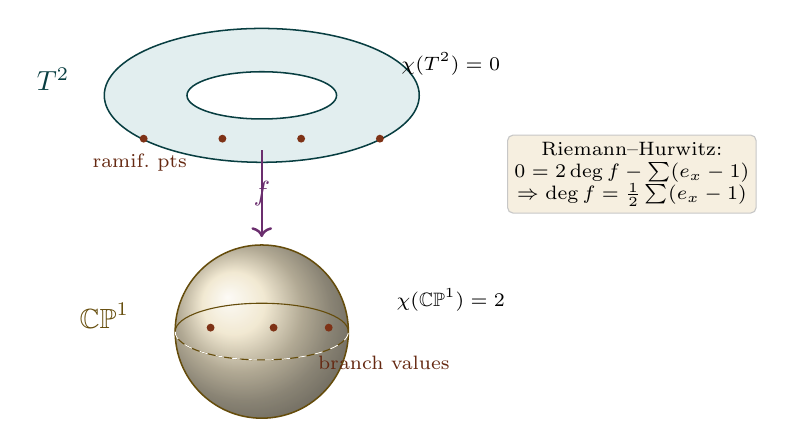
\begin{tikzpicture}[scale=1.0, every node/.style={font=\scriptsize}]
% Top: torus drawn as donut shape
\begin{scope}[yshift=2.2cm]
  \filldraw[draw=formteal!55!black, fill=formteal!12, line width=0.55pt] (0,0) ellipse (2.0 and 0.85);
  \fill[white] (0,0) ellipse (0.95 and 0.3);
  \draw[formteal!55!black, line width=0.55pt] (0,0) ellipse (0.95 and 0.3);
  % Ramification points
  \foreach \xx in {-1.5,-0.5,0.5,1.5}{
    \fill[formrust!75!black] (\xx,-0.55) circle (0.05);
  }
  \node[formteal!55!black, font=\bfseries] at (-2.65,0.2) {$T^2$};
  \node[formrust!60!black, font=\scriptsize] at (-1.55,-0.85) {ramif.\ pts};
  \node[font=\scriptsize] at (2.4,0.4) {$\chi(T^2)=0$};
\end{scope}
% Map arrow
\node[formplum, font=\bfseries] at (0,0.95) {$f$};
\draw[->, formplum, line width=0.9pt] (0,1.5) -- (0,0.4);
% Bottom: CP^1 sphere
\begin{scope}[yshift=-0.8cm]
  \shade[ball color=formgold!30, opacity=0.85] (0,0) circle (1.1);
  \draw[formgold!55!black, line width=0.55pt] (0,0) circle (1.1);
  \draw[formgold!55!black, line width=0.4pt] (0,0) ellipse (1.1 and 0.36);
  \draw[dashed, white, line width=0.35pt] (-1.1,0) arc (180:360:1.1 and 0.36);
  \foreach \xx in {-0.65,0.15,0.85}{
    \fill[formrust!75!black] (\xx,0.05) circle (0.05);
  }
  \node[formgold!55!black, font=\bfseries] at (-2.0,0.2) {$\CP^1$};
  \node[formrust!60!black, font=\scriptsize] at (1.55,-0.4) {branch values};
  \node[font=\scriptsize] at (2.4,0.4) {$\chi(\CP^1)=2$};
\end{scope}
% Riemann-Hurwitz annotation
\node[font=\scriptsize, align=center, fill=formivory, rounded corners=2pt, inner sep=2.5pt, draw=black!22]
  at (4.7,1.2) {Riemann--Hurwitz:\\$0=2\deg f-\sum(e_x-1)$\\$\Rightarrow\deg f=\tfrac12\sum(e_x-1)$};
\end{tikzpicture}
\visualcaption{Maps from the torus to the sphere are always branched. Riemann--Hurwitz turns the topological mismatch $\chi(T^2)=0\neq 2\deg f=\chi(\CP^1)\cdot\deg f$ into the equality between $2\deg f$ and the total ramification.}
\end{center}

\section*{Problem 7: Fundamental Theorem of Algebra}

\begin{intentrequirements}
\item \textbf{Intent.} Prove the Fundamental Theorem of Algebra using the compact Riemann surface proposition rather than Liouville's theorem or elementary estimates.
\item \textbf{Required outputs.} Extend a nonconstant polynomial $p$ to a holomorphic map $P:\CP^1\to\CP^1$, prove the extension is holomorphic at $\infty$, use surjectivity to find a preimage of $0$, and conclude that $p$ has a complex root.
\item \textbf{Required explanations.} In the coordinate $w=1/z$, show that $1/p(1/w)$ is holomorphic near $w=0$ and vanishes there, so $P(\infty)=\infty$.
\item \textbf{Common pitfalls to avoid.} Surjectivity gives a point mapping to $0$ in $\CP^1$, but one must also note it is not $\infty$, since $P(\infty)=\infty$.
\end{intentrequirements}

\windingnote{The classical winding-number proof of the Fundamental Theorem of Algebra reads: for $p(z)=z^n+\dots$, the winding number of $p$ around $0$ along the circle $|z|=R$ is $\frac{1}{2\pi i}\oint_{|z|=R}\frac{p'(z)}{p(z)}\,dz$, which for large $R$ equals $n$ (since $p\sim z^n$ and $p'/p\sim n/z$, with $\oint dz/z=2\pi i$). A winding number $n>0$ around $0$ forces $p^{-1}(0)$ to contain $n$ points counted with multiplicity. The Riemann-surface proof in this problem is the same idea in different dress: $P:\CP^1\to\CP^1$ has degree $n$ (the global winding of $p$), surjectivity gives a $0$-fiber of size $n$, hence $n$ roots. The winding form $dp/p$ counts roots through its residue sum.}

\handsketch{%
\fill[handpaper] (-3.4,-1.9) rectangle (3.4,1.9);
\draw[hand] (-3.4,-1.9) rectangle (3.4,1.9);
% Big circle |z|=R
\begin{scope}[xshift=-1.85cm]
  \draw[handthick] (0,0) circle (1.0);
  \node[handnote] at (0,1.2) {$|z|=R$ large};
  \draw[draw=handink, line width=0.55pt, -{Latex[length=1.7mm]}] (50:1.0) arc (50:130:1.0);
\end{scope}
% Map p(z)
\draw[draw=handink, line width=0.8pt, -{Latex[length=2.5mm]}] (-0.7,0) -- (0.55,0);
\node[handnote] at (-0.1,0.3) {$p(z)\sim z^n$};
% Right: image, wraps n times
\begin{scope}[xshift=1.85cm]
  \draw[draw=handink, line width=0.6pt, smooth, samples=120, variable=\t, domain=0:1080]
    plot ({(0.85+0.05*sin(6*\t))*cos(\t)},{(0.85+0.05*sin(6*\t))*sin(\t)});
  \fill[handink] (0,0) circle (0.05);
  \node[handnote] at (0.16,-0.18) {$0$};
  \node[handnote] at (0,1.2) {winding $=n$};
\end{scope}
\node[handnote] at (0,-1.4) {$\dfrac{1}{2\pi i}\oint\dfrac{p'\,dz}{p}=n=\deg p$};
\node[handnote] at (0,-1.85) {hence $n$ roots};
}

\textbf{Theorem.}
Every nonconstant polynomial $p(z)\in\C[z]$ has a zero in $\C$. Equivalently, every polynomial of degree $n\geq1$ factors over $\C$ as a product of $n$ linear factors, counted with multiplicity.

\textbf{Proof using compact Riemann surfaces.}
Let $p(z)$ be a nonconstant polynomial. It defines a meromorphic function on $\CP^1$ with a pole at $\infty$. Equivalently, it defines a holomorphic map
\[
 P:\CP^1\to\CP^1
\]
by setting $P(z)=p(z)$ on the affine chart $\C$ and $P(\infty)=\infty$.
This extension is holomorphic at $\infty$: in the coordinate $w=1/z$, a degree $n$ polynomial has the form
\[
 p(1/w)=a_nw^{-n}+\cdots,
\]
so the target coordinate $1/P$ is holomorphic and vanishes at $w=0$.

The map $P$ is nonconstant. By the proposition in Problem 5, a nonconstant holomorphic map between compact Riemann surfaces is surjective. Therefore $0\in\CP^1$ is in the image of $P$.
Since $P(\infty)=\infty\neq0$, the point mapping to $0$ must be some finite $z_0\in\C$. Thus
\[
 p(z_0)=0.
\]
This proves that every nonconstant complex polynomial has a complex root. Repeatedly dividing by linear factors gives the full factorization into linear factors.

\begin{center}
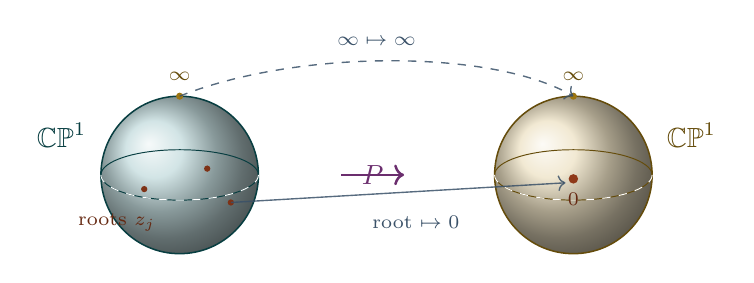
\begin{tikzpicture}[scale=1.0, every node/.style={font=\scriptsize}]
% Source CP^1
\begin{scope}
  \shade[ball color=formteal!25] (0,0) circle (1.0);
  \draw[formteal!55!black, line width=0.55pt] (0,0) circle (1.0);
  \draw[formteal!55!black, line width=0.35pt] (0,0) ellipse (1.0 and 0.32);
  \draw[dashed, white, line width=0.35pt] (-1.0,0) arc (180:360:1.0 and 0.32);
  \fill[formgold!85!black] (0,1.0) circle (0.045);
  \node[formgold!55!black, font=\scriptsize] at (0,1.25) {$\infty$};
  \fill[formrust!75!black] (-0.45,-0.18) circle (0.04);
  \fill[formrust!75!black] (0.35,0.08) circle (0.04);
  \fill[formrust!75!black] (0.65,-0.35) circle (0.04);
  \node[formrust!60!black, font=\scriptsize] at (-0.8,-0.6) {roots $z_j$};
  \node[formteal!55!black, font=\bfseries] at (-1.5,0.5) {$\CP^1$};
\end{scope}
% Map
\node[formplum, font=\bfseries] at (2.45,0) {$P$};
\draw[->, formplum, line width=0.9pt] (2.05,0) -- (2.85,0);
% Target CP^1
\begin{scope}[xshift=5.0cm]
  \shade[ball color=formgold!25] (0,0) circle (1.0);
  \draw[formgold!55!black, line width=0.55pt] (0,0) circle (1.0);
  \draw[formgold!55!black, line width=0.35pt] (0,0) ellipse (1.0 and 0.32);
  \draw[dashed, white, line width=0.35pt] (-1.0,0) arc (180:360:1.0 and 0.32);
  \fill[formgold!85!black] (0,1.0) circle (0.045);
  \node[formgold!55!black, font=\scriptsize] at (0,1.25) {$\infty$};
  \fill[formrust!85!black] (0,-0.05) circle (0.06);
  \node[formrust!60!black, font=\scriptsize, below] at (0,-0.1) {$0$};
  \node[formgold!55!black, font=\bfseries] at (1.5,0.5) {$\CP^1$};
\end{scope}
% Map sends roots to 0, and infinity to infinity
\draw[->, formslate, line width=0.5pt, opacity=0.85, dashed]
  (0,1.0) .. controls (1.5,1.6) and (4.0,1.6) .. (5.0,1.0);
\node[formslate, font=\scriptsize] at (2.5,1.7) {$\infty\mapsto\infty$};
\draw[->, formslate, line width=0.5pt, opacity=0.85] (0.65,-0.35) -- (4.9,-0.1);
\node[formslate, font=\scriptsize] at (3.0,-0.6) {root $\mapsto 0$};
\end{tikzpicture}
\visualcaption{A nonconstant polynomial extends to a holomorphic self-map $P:\CP^1\to\CP^1$ sending $\infty\to\infty$. Surjectivity (open mapping plus compact-Hausdorff) forces $0$ to be in the image, and its preimage must be a finite point, hence a root of the polynomial.}
\end{center}

\section*{Problem 8: Residues of Meromorphic $1$-Forms on a Compact Riemann Surface}

\begin{intentrequirements}
\item \textbf{Intent.} Prove that residues of meromorphic $1$-forms are intrinsic and that their total sum on a compact Riemann surface is zero.
\item \textbf{Required outputs.} Prove coordinate independence of $\Res_p(\omega)$ and prove
\[
 \sum_j\Res_{p_j}(\omega)=0
\]
for all poles $p_j$ of $\omega$.
\item \textbf{Required explanations.} For coordinate independence, identify the residue with $\frac{1}{2\pi i}\int_\gamma\omega$ around a small loop. For the sum formula, remove small disks around all poles and apply Stokes to the punctured compact surface.
\item \textbf{Common pitfalls to avoid.} The boundary circles of the punctured surface have the negative orientation relative to the usual positively oriented boundaries of the removed disks.
\end{intentrequirements}

\windingnote{This is the full upgrade of Problem~2 to a compact Riemann surface. The residue $\Res_p(\omega)=\frac{1}{2\pi i}\oint_\gamma\omega$ is exactly the winding integral of $\omega$ around the pole $p$, divided by $2\pi i$; coordinate-independence of the residue is the coordinate-independence of the winding integral. The sum-of-residues theorem $\sum_p\Res_p(\omega)=0$ is the global compatibility forced by the absence of a global ``argument'' obstruction on a compact closed surface: there is nowhere for the total winding to escape. On the plane, the winding form would integrate to $2\pi i$ around a single pole; on a compact surface, every pole must be cancelled by another pole somewhere else, which is why $\deg(f)=0$ for principal divisors (Problem~9) and $\deg(\omega)=2g-2$ for canonical divisors (Problem~12) are forced.}

\handsketch{%
\fill[handpaper] (-3.4,-1.9) rectangle (3.4,1.9);
\draw[hand] (-3.4,-1.9) rectangle (3.4,1.9);
% Compact surface (genus 2 schematic)
\draw[handthick] plot[smooth cycle] coordinates {(-3.0,-0.55) (-2.55,0.7) (-1.3,0.95) (0.0,0.7) (1.3,0.95) (2.55,0.7) (3.0,-0.55) (1.5,-1.1) (-1.5,-1.1)};
% Handles
\fill[white] (-1.2,0.15) ellipse (0.35 and 0.1);
\draw[draw=handink, line width=0.55pt] (-1.2,0.15) ellipse (0.35 and 0.1);
\fill[white] (1.2,0.15) ellipse (0.35 and 0.1);
\draw[draw=handink, line width=0.55pt] (1.2,0.15) ellipse (0.35 and 0.1);
% Poles with residues
\foreach \xx/\yy/\res in {-2.0/0.4/+2, -0.3/-0.5/-1, 0.8/0.55/-3, 2.1/-0.45/+2}{
  \draw[draw=handink, line width=0.55pt] (\xx,\yy) circle (0.18);
  \fill[handink] (\xx,\yy) circle (0.04);
  \node[handnote] at (\xx,\yy-0.4) {$\res$};
}
\node[handnote] at (-3.0,1.0) {$M$};
\node[handnote] at (0,-1.55) {$\sum \mathrm{Res}_p(\omega)=0$};
\node[handnote] at (0,-1.85) {(no place for winding to escape)};
}

\subsection*{Problem 8-1: Coordinate independence of the residue $\Res_p(\omega)$}

Suppose $p\in M$ is a pole. In a local coordinate $z$ with $z(p)=0$, write
\[
 \omega=f(z)\,dz,\qquad
 f(z)=\sum_{n=-m}^{\infty}a_nz^n.
\]
The residue is defined as
\[
 \Res_p(\omega)=a_{-1}.
\]
Equivalently, for $r>0$ sufficiently small that the closed disk $|z|\leq r$ contains no pole other than $p$,
\[
 \Res_p(\omega)=\frac{1}{2\pi i}\int_{|z|=r}\omega.
\]
Indeed, termwise integration of the Laurent series gives
\[
 \int_{|z|=r}f(z)\,dz
 =\sum_{n=-m}^\infty a_n\int_{|z|=r}z^n\,dz
 =2\pi i\,a_{-1},
\]
since $\int_{|z|=r}z^n\,dz=0$ for $n\neq-1$.

The integral of a $1$-form around a small positively oriented loop is intrinsic: it depends only on $\omega$ and the loop, not on the coordinate used to write $\omega$. Therefore the value $a_{-1}$ recovered from the integral is independent of the local coordinate, so $\Res_p(\omega)$ is well defined.

\subsection*{Problem 8-2: The sum of residues vanishes}

Let $p_1,\dots,p_n$ be the poles of $\omega$. Choose pairwise disjoint coordinate disks $B_j$ around $p_j$, sufficiently small that $\omega$ has no pole on the boundary circles, and set
\[
 M_\eps=M\setminus\bigcup_{j=1}^n B_j.
\]
On $M_\eps$ the form $\omega$ is holomorphic. Locally $\omega=f(z)\,dz$ with $f$ holomorphic, so
\[
 d\omega=df\wedge dz=0
\]
on $M_\eps$. By the generalized Stokes theorem,
\[
 0=\int_{M_\eps}d\omega=\int_{\partial M_\eps}\omega.
\]
Since $M$ is closed (no boundary), $\partial M_\eps=-\bigsqcup_{j=1}^n \partial B_j$ with each $\partial B_j$ in the orientation opposite to its usual positive (counterclockwise) orientation as the boundary of $B_j$. Hence
\[
 \int_{\partial M_\eps}\omega
 =
 -\sum_{j=1}^n\int_{\partial B_j}\omega
 =
 -2\pi i\sum_{j=1}^n\Res_{p_j}(\omega),
\]
using 8-1 in the last step. Therefore
\[
 \sum_{j=1}^n\Res_{p_j}(\omega)=0.
\]

\begin{center}
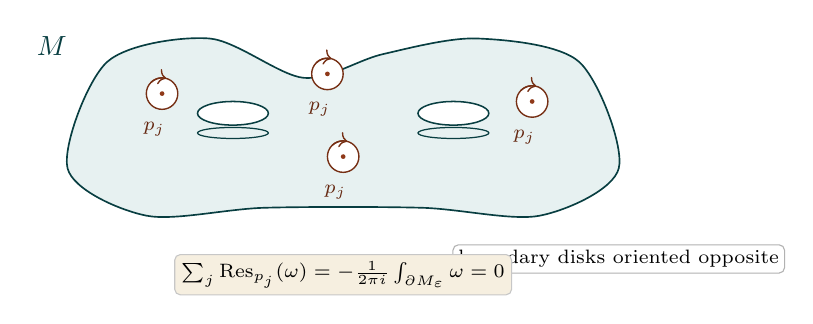
\begin{tikzpicture}[scale=1.0, every node/.style={font=\scriptsize}]
% Genus-2 surface drawn schematically
\draw[draw=formteal!55!black, fill=formteal!10, line width=0.6pt]
  plot[smooth cycle] coordinates
  {(-3.5,-0.5) (-3.0,0.85) (-1.7,1.15) (-0.5,0.65) (0.5,0.95) (1.7,1.15) (3.0,0.85) (3.5,-0.5) (2.5,-1.1) (1.0,-1.0) (-1.0,-1.0) (-2.5,-1.1)};
% Two handles
\filldraw[draw=formteal!55!black, fill=white, line width=0.55pt] (-1.4,0.2) ellipse (0.45 and 0.15);
\filldraw[draw=formteal!55!black, fill=white, line width=0.55pt] (1.4,0.2) ellipse (0.45 and 0.15);
\draw[formteal!55!black, line width=0.45pt] (-1.4,-0.05) ellipse (0.45 and 0.07);
\draw[formteal!55!black, line width=0.45pt] (1.4,-0.05) ellipse (0.45 and 0.07);
% Poles with small disks deleted
\foreach \xx/\yy in {-2.3/0.45, 0.0/-0.35, 2.4/0.35, -0.2/0.7}{
  \filldraw[draw=formrust!70!black, fill=white, line width=0.5pt] (\xx,\yy) circle (0.20);
  \draw[->, formrust!70!black, line width=0.5pt] ($(\xx,\yy)+(135:0.20)$) arc (135:75:0.20);
  \fill[formrust!85!black] (\xx,\yy) circle (0.03);
  \node[formrust!60!black, font=\scriptsize] at (\xx-0.1,\yy-0.45) {$p_j$};
}
% Annotations
\node[formteal!55!black, font=\bfseries] at (-3.7,1.05) {$M$};
\node[font=\scriptsize, fill=white, rounded corners=2pt, inner sep=2pt, draw=black!30]
  at (3.5,-1.65) {boundary disks oriented opposite};
\node[font=\scriptsize, fill=formivory, rounded corners=2pt, inner sep=2.5pt, draw=black!22]
  at (0,-1.85) {$\sum_j \Res_{p_j}(\omega)=-\frac{1}{2\pi i}\int_{\partial M_\eps}\omega=0$};
\end{tikzpicture}
\visualcaption{On a compact Riemann surface, removing tiny disks around the poles leaves a manifold-with-boundary on which $d\omega=0$. Stokes' theorem then forces the sum of all residues to vanish. The induced inner-boundary orientation provides the sign.}
\end{center}

\section*{Problem 9: Residue Theorem and the Degree of a Principal Divisor}

\begin{intentrequirements}
\item \textbf{Intent.} Deduce that every principal divisor on a compact Riemann surface has degree zero by applying the residue theorem to the logarithmic derivative $df/f$.
\item \textbf{Required outputs.} Consider $\omega=df/f$, prove $\sum_p\Res_p(df/f)=0$, compute locally that
\[
 \Res_p(df/f)=\nu_p(f),
\]
and conclude $\sum_p\nu_p(f)=0$.
\item \textbf{Required explanations.} In a local coordinate write $f=z^m u(z)$ with $u(0)\neq0$, then compute
\[
 df/f=m\,dz/z+du/u.
\]
\item \textbf{Common pitfalls to avoid.} The integer $m$ can be positive, negative, or zero. The same computation handles zeros, poles, and ordinary nonzero points.
\end{intentrequirements}

\windingnote{The logarithmic derivative $df/f$ is the winding form pulled back along $f$: $df/f=f^*(dw/w)$, where $dw/w$ is the meromorphic version of the winding form on $\C^*\subset\CP^1$. Locally near a point of order $m=\nu_p(f)$, $f=z^m u(z)$ with $u(0)\neq 0$, so $df/f=m\,dz/z+du/u$. The first term is $m$ times the winding form at $p$ --- meaning $f$ wraps the value $0$ exactly $m$ times around $p$ --- and the second term is holomorphic, hence has zero residue. The constraint $\sum_p\nu_p(f)=\deg(f)=0$ is the residue theorem for the pull-back winding form. Geometrically: on a compact Riemann surface, every $f$ must wind around $0$ as many times positively as negatively, otherwise the total angular accumulation would not close up.}

\handsketch{%
\fill[handpaper] (-3.4,-1.9) rectangle (3.4,1.9);
\draw[hand] (-3.4,-1.9) rectangle (3.4,1.9);
\draw[handthick] plot[smooth cycle] coordinates {(-3.0,-0.7) (-2.5,0.7) (-1.0,1.0) (0.7,1.0) (2.4,0.7) (3.0,-0.7) (1.4,-1.15) (-1.4,-1.15)};
% Zeros: positive residues
\foreach \xx/\yy/\res in {-2.0/0.3/+2, 0.1/0.5/+1}{
  \fill[handink] (\xx,\yy) circle (0.06);
  \draw[draw=handink, line width=0.45pt, -{Latex[length=1.5mm]}] ($(\xx,\yy)+(35:0.22)$) arc (35:300:0.22);
  \node[handnote] at (\xx+0.32,\yy+0.05) {$\res$};
}
% Poles: negative residues
\foreach \xx/\yy/\res in {-0.8/-0.45/-2, 1.8/-0.4/-1}{
  \draw[draw=handink, line width=0.55pt] (\xx,\yy) circle (0.1);
  \fill[white] (\xx,\yy) circle (0.1);
  \fill[handink] (\xx,\yy) circle (0.03);
  \draw[draw=handink, line width=0.45pt, dashed, -{Latex[length=1.5mm]}] ($(\xx,\yy)+(35:0.22)$) arc (35:300:0.22);
  \node[handnote] at (\xx+0.32,\yy+0.05) {$\res$};
}
\node[handnote] at (0,1.4) {$df/f=f^*(dw/w)$};
\node[handnote] at (0,-1.55) {$\sum\nu_p(f)=2+1-2-1=0$};
}

Let $M$ be compact and let $f$ be a nonzero meromorphic function on $M$. The principal divisor is
\[
 (f)=\sum_{p\in M}\nu_p(f)\,p,
\]
where $\nu_p(f)=\ord_p(f)$.
We prove
\[
 \deg(f)=\sum_{p\in M}\nu_p(f)=0.
\]

Consider the meromorphic $1$-form
\[
 \omega=\frac{df}{f}.
\]
By Problem 8,
\[
 \sum_{p\in M}\Res_p\left(\frac{df}{f}\right)=0.
\]
It remains to identify the residue with the order of $f$.

Choose a local coordinate $z$ centered at $p$. Write
\[
 f(z)=z^m u(z),
\]
where $m=\nu_p(f)$ and $u(0)\neq0$ is holomorphic and nonzero near $0$. Then
\[
 \frac{df}{f}
 =
 \frac{d(z^m u)}{z^m u}
 =
 m\frac{dz}{z}+\frac{du}{u}.
\]
The form $du/u$ is holomorphic near $p$, so it has residue $0$. Hence
\[
 \Res_p\left(\frac{df}{f}\right)=m=\nu_p(f).
\]
Therefore
\[
 0=\sum_{p\in M}\Res_p\left(\frac{df}{f}\right)
 =
 \sum_{p\in M}\nu_p(f)
 =
 \deg(f).
\]

\begin{center}
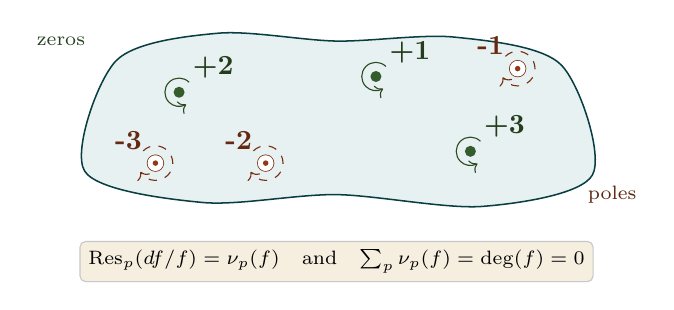
\begin{tikzpicture}[scale=1.0, every node/.style={font=\scriptsize}]
% Surface
\filldraw[draw=formteal!55!black, fill=formteal!10, line width=0.55pt]
  plot[smooth cycle] coordinates {(-3.2,-0.7) (-2.8,0.7) (-1.5,1.05) (0,0.95) (1.5,1.0) (2.85,0.65) (3.25,-0.75) (1.85,-1.15) (0,-1.0) (-1.7,-1.1)};
% Zeros: marked with green dots and "+m" labels
\foreach \xx/\yy/\m in {-2.0/0.3/+2, 0.5/0.5/+1, 1.7/-0.45/+3}{
  \fill[formsage!75!black] (\xx,\yy) circle (0.07);
  \draw[->, formsage!60!black, line width=0.4pt] ($(\xx,\yy)+(45:0.18)$) arc (45:300:0.18);
  \node[formsage!50!black, font=\bfseries, above right] at (\xx+0.05,\yy+0.05) {\m};
}
% Poles: marked with red rings and "-m" labels
\foreach \xx/\yy/\m in {-0.9/-0.6/-2, 2.3/0.6/-1, -2.3/-0.6/-3}{
  \draw[formrust!70!black, line width=0.55pt] (\xx,\yy) circle (0.10);
  \fill[white] (\xx,\yy) circle (0.10);
  \fill[formrust!85!black] (\xx,\yy) circle (0.035);
  \draw[->, formrust!70!black, line width=0.4pt, dashed] ($(\xx,\yy)+(135:0.22)$) arc (135:-150:0.22);
  \node[formrust!60!black, font=\bfseries, above left] at (\xx-0.05,\yy+0.05) {\m};
}
% Caption
\node[font=\scriptsize, formsage!55!black] at (-3.5,0.95) {zeros};
\node[font=\scriptsize, formrust!55!black] at (3.5,-1.0) {poles};
\node[font=\scriptsize, align=center, fill=formivory, rounded corners=2pt, inner sep=3pt, draw=black!22]
  at (0,-1.85) {$\Res_p(df/f)=\nu_p(f)$\quad and\quad $\sum_p \nu_p(f)=\deg(f)=0$};
\end{tikzpicture}
\visualcaption{The logarithmic derivative $df/f$ has simple poles at every zero and pole of $f$, with residue equal to the signed order. The vanishing of the residue sum is exactly the degree-zero condition for principal divisors.}
\end{center}

\section*{Problem 10: Principal Divisor on $\CP^1$ and the Canonical Divisor of $dz$}

\begin{intentrequirements}
\item \textbf{Intent.} Compute two explicit divisors on $\CP^1$: a principal divisor of a rational function and the divisor of the meromorphic differential $dz$.
\item \textbf{Required outputs.} Compute the finite orders at $0$, $1$, and $2$, check the contribution at $\infty$, verify $\deg(f)=0$, extend $dz$ to $\CP^1$, and show
\[
 (dz)=-2[\infty],\qquad \deg(dz)=-2.
\]
\item \textbf{Required explanations.} Use the coordinate $w=1/z$ at infinity. For the function, compute $f(1/w)$; for the differential, compute $dz=d(w^{-1})=-w^{-2}dw$.
\item \textbf{Common pitfalls to avoid.} Do not forget infinity. Rational functions and differentials on $\CP^1$ almost always have essential divisor information at $\infty$.
\end{intentrequirements}

\windingnote{This is the simplest non-trivial case of Problem~9. The function $f(z)=z^2(z-1)/(z-2)^3$ has, by direct computation, $df/f=\frac{2\,dz}{z}+\frac{dz}{z-1}-\frac{3\,dz}{z-2}+\text{regular at }\infty$. Each $dz/(z-a)$ is the winding form $dz/z$ translated to base point $a$, with residue $1$; the coefficients $\{2,+1,-3\}$ are the orders $\{2,1,-3\}$ in the divisor and sum to $0$, confirming the global winding-residue constraint. For the form $dz$, the divisor $(dz)=-2[\infty]$ records that $dz$ has a pole of order $2$ at $\infty$ but no zero or pole on the finite chart --- which is consistent with $\deg(dz)=2g-2=-2$ on the sphere.}

\handsketch{%
\fill[handpaper] (-3.4,-1.9) rectangle (3.4,1.9);
\draw[hand] (-3.4,-1.9) rectangle (3.4,1.9);
% CP^1 sphere
\draw[handthick] (0,0) circle (1.45);
\draw[draw=handink, line width=0.4pt, opacity=0.45] (0,0) ellipse (1.45 and 0.45);
% Four marked points
\fill[handink] (200:1.45) circle (0.07);
\node[handnote, anchor=east] at ($(200:1.45)+(180:0.15)$) {$z=0$};
\node[handnote] at ($(200:1.45)+(220:0.4)$) {$+2$};
\fill[handink] (340:1.45) circle (0.07);
\node[handnote, anchor=west] at ($(340:1.45)+(0:0.15)$) {$z=1$};
\node[handnote] at ($(340:1.45)+(320:0.4)$) {$+1$};
\fill[handink] (15:1.45) circle (0.07);
\node[handnote, anchor=west] at ($(15:1.45)+(0:0.15)$) {$z=2$};
\node[handnote] at ($(15:1.45)+(45:0.4)$) {$-3$};
\fill[handink] (90:1.45) circle (0.07);
\node[handnote] at ($(90:1.45)+(90:0.2)$) {$\infty$};
\node[handnote] at ($(90:1.45)+(90:0.5)$) {$0$};
\node[handnote] at (0,0) {$(f)$};
\node[handnote] at (0,-1.85) {$\deg(f)=2+1-3+0=0$};
}

Let
\[
 f(z)=\frac{z^2(z-1)}{(z-2)^3}.
\]
On the affine chart $\C\subset\CP^1$, the zeros and poles are clear:
\[
 \ord_0(f)=2,\qquad
 \ord_1(f)=1,\qquad
 \ord_2(f)=-3.
\]
To compute the contribution at $\infty$, use the coordinate $w=1/z$. Then
\[
 f(1/w)
 =
 \frac{w^{-2}(w^{-1}-1)}{(w^{-1}-2)^3}
 =
 \frac{1-w}{(1-2w)^3}.
\]
This is holomorphic and nonzero at $w=0$, so
\[
 \ord_\infty(f)=0.
\]
Thus
\[
 (f)=2[0]+[1]-3[2].
\]
The degree is
\[
 \deg(f)=2+1-3=0,
\]
as expected for a principal divisor.

Now consider the meromorphic $1$-form $dz$ on $\C\subset\CP^1$. It has no zeros or poles on the finite chart. Near $\infty$, again set $w=1/z$. Then
\[
 dz=d(w^{-1})=-w^{-2}\,dw.
\]
So $dz$ has a pole of order $2$ at $\infty$. Therefore
\[
 (dz)=-2[\infty],
\]
and hence
\[
 \deg(dz)=-2.
\]

\begin{center}
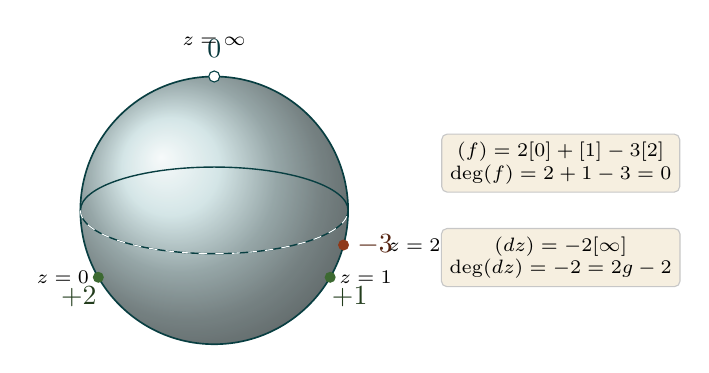
\begin{tikzpicture}[scale=1.0, every node/.style={font=\scriptsize}]
% Riemann sphere with 4 marked points
\shade[ball color=formteal!28, opacity=0.85] (0,0) circle (1.7);
\draw[formteal!55!black, line width=0.6pt] (0,0) circle (1.7);
\draw[formteal!55!black, line width=0.5pt] (0,0) ellipse (1.7 and 0.55);
\draw[dashed, white, line width=0.4pt] (-1.7,0) arc (180:360:1.7 and 0.55);
% Points: 0, 1, 2, infinity
\coordinate (Z0) at (210:1.7);
\coordinate (Z1) at (330:1.7);
\coordinate (Z2) at (-15:1.7);
\coordinate (ZI) at (90:1.7);
\fill[formsage!85!black] (Z0) circle (0.07);
\fill[formsage!85!black] (Z1) circle (0.07);
\fill[formrust!85!black] (Z2) circle (0.07);
\fill[white] (ZI) circle (0.07);
\draw[formteal!60!black] (ZI) circle (0.07);
% Multiplicities
\node[formsage!50!black, font=\bfseries] at ($(Z0)+(225:0.35)$) {$+2$};
\node[formsage!50!black, font=\bfseries] at ($(Z1)+(315:0.35)$) {$+1$};
\node[formrust!50!black, font=\bfseries] at ($(Z2)+(0:0.4)$) {$-3$};
\node[formteal!50!black, font=\bfseries] at ($(ZI)+(90:0.35)$) {$0$};
% Labels
\node[font=\scriptsize] at ($(Z0)+(180:0.45)$) {$z=0$};
\node[font=\scriptsize] at ($(Z1)+(0:0.45)$) {$z=1$};
\node[font=\scriptsize] at ($(Z2)+(0:0.4)+(0:0.5)$) {$z=2$};
\node[font=\scriptsize] at ($(ZI)+(90:0.45)$) {$z=\infty$};
% Right side: divisor and degree
\node[font=\scriptsize, align=center, fill=formivory, rounded corners=2pt, inner sep=3pt, draw=black!22]
  at (4.4,0.6) {$(f)=2[0]+[1]-3[2]$\\$\deg(f)=2+1-3=0$};
\node[font=\scriptsize, align=center, fill=formivory, rounded corners=2pt, inner sep=3pt, draw=black!22]
  at (4.4,-0.6) {$(dz)=-2[\infty]$\\$\deg(dz)=-2=2g-2$};
\end{tikzpicture}
\visualcaption{Each marked point on the Riemann sphere carries an integer order. The principal divisor of $f$ has degree zero (zeros and poles balance), while the canonical divisor of $dz$ has degree $-2=2g-2$, matching the genus formula on $\CP^1$.}
\end{center}

\section*{Problem 11: Riemann-Hurwitz Theorem}

\begin{intentrequirements}
\item \textbf{Intent.} State and prove the Riemann--Hurwitz theorem relating Euler characteristics, degree, and ramification for a nonconstant holomorphic map of compact Riemann surfaces.
\item \textbf{Required outputs.} State
\[
 \chi(X)=n\chi(Y)-\sum_{x\in X}(e_x(f)-1),
\]
where $n=\deg f$, and prove it by comparing triangulations.
\item \textbf{Required explanations.} Explain why edges and faces lift $n$ times, while vertices over branch values contribute the correction term
\[
 \#f^{-1}(y)=n-\sum_{x\in f^{-1}(y)}(e_x-1).
\]
\item \textbf{Common pitfalls to avoid.} The ramification correction is subtracted in the Euler characteristic formula for $\chi(X)$ and added in the genus form
\[
 2g_X-2=n(2g_Y-2)+\sum_x(e_x-1).
\]
\end{intentrequirements}

\windingnote{Riemann--Hurwitz expresses, in one identity, both Gauss--Bonnet's winding count (via $\chi$) and the residue-sum theorem for the pull-back of the winding form (via $\sum e_x$). To see the bridge: take any nonzero meromorphic $1$-form $\eta$ on $Y$; its divisor has $\deg(\eta)=2g_Y-2$. The pull-back $f^*\eta$ has divisor $(f^*\eta)=f^*(\eta)+R$, where $R=\sum_{x\in X}(e_x-1)x$ is the ramification divisor. Taking degrees: $\deg(f^*\eta)=n\deg(\eta)+\deg(R)$. But the left side equals $2g_X-2$ on $X$, so $2g_X-2=n(2g_Y-2)+\sum_x(e_x-1)$. The whole proof rests on the additivity of winding orders under pull-back --- exactly the local property $f^*(dw/w)=e_x\,dz/z+\text{regular}$.}

\handsketch{%
\fill[handpaper] (-3.4,-1.9) rectangle (3.4,1.9);
\draw[hand] (-3.4,-1.9) rectangle (3.4,1.9);
% Top: triangulation of X with one ramification
\begin{scope}[yshift=0.85cm]
  \draw[handthick] (-2.6,-0.55) rectangle (2.6,0.55);
  % triangle grid
  \draw[draw=handink, line width=0.35pt] (-2.3,-0.4) -- (-1.3,-0.4) -- (-1.8,0.4) -- cycle;
  \draw[draw=handink, line width=0.35pt] (-1.8,0.4) -- (-0.8,0.4) -- (-1.3,-0.4);
  \draw[draw=handink, line width=0.35pt] (-0.8,0.4) -- (-0.3,-0.4) -- (-1.3,-0.4);
  \draw[draw=handink, line width=0.35pt] (-0.3,-0.4) -- (0.7,-0.4) -- (0.2,0.4);
  \draw[draw=handink, line width=0.35pt] (0.7,-0.4) -- (1.2,0.4) -- (0.2,0.4);
  % ramif point
  \fill[handink] (1.8,0) circle (0.06);
  \draw[draw=handink, line width=0.5pt] (1.8,0) circle (0.15);
  \node[handnote] at (1.8,0.35) {$e=2$};
  \node[handnote] at (-3.0,0.05) {$X$};
\end{scope}
% Arrow
\draw[draw=handink, line width=0.8pt, -{Latex[length=2.5mm]}] (0,0.2) -- (0,-0.2);
\node[handnote] at (0.3,-0.05) {$f$};
% Bottom: Y triangulation
\begin{scope}[yshift=-0.85cm]
  \draw[handthick] (-2.6,-0.55) rectangle (2.6,0.55);
  \draw[draw=handink, line width=0.35pt] (-2.3,-0.3) -- (-1.3,-0.3) -- (-1.8,0.35) -- cycle;
  \draw[draw=handink, line width=0.35pt] (-0.5,-0.3) -- (0.5,-0.3) -- (0.0,0.35) -- cycle;
  \draw[draw=handink, line width=0.35pt] (1.0,-0.3) -- (2.0,-0.3) -- (1.5,0.35) -- cycle;
  % Branch value at one vertex
  \fill[handink] (1.5,0.35) circle (0.06);
  \node[handnote] at (1.5,0.55) {branch};
  \node[handnote] at (-3.0,0.05) {$Y$};
\end{scope}
\node[handnote] at (0,-1.85) {edges/faces lift $n\times$, vertices lose $(e_x-1)$};
}

\textbf{Theorem.}
Let
\[
 f:X\to Y
\]
be a nonconstant holomorphic map of degree $n$ between compact Riemann surfaces. Let $e_x(f)$ be the ramification index at $x\in X$. Then
\[
 \boxed{\chi(X)=n\chi(Y)-\sum_{x\in X}(e_x(f)-1).}
\]
Equivalently, in terms of genera,
\[
 2g_X-2=n(2g_Y-2)+\sum_{x\in X}(e_x(f)-1).
\]

\textbf{Proof.}
Choose a triangulation of $Y$ such that every branch value of $f$ is a vertex. Pull this triangulation back to $X$.

Let $V_Y,E_Y,F_Y$ be the numbers of vertices, edges, and faces of the triangulation of $Y$. Away from branch values, the map is an $n$-sheeted covering. Therefore every edge and every face of $Y$ has exactly $n$ lifts:
\[
 E_X=nE_Y,\qquad F_X=nF_Y.
\]

For vertices, there is a correction from ramification. For a vertex $y\in Y$,
\[
 \sum_{x\in f^{-1}(y)}e_x(f)=n.
\]
Therefore
\[
 \# f^{-1}(y)
 =
 n-\sum_{x\in f^{-1}(y)}(e_x(f)-1).
\]
Summing over all vertices gives
\[
 V_X=nV_Y-\sum_{x\in X}(e_x(f)-1),
\]
because ramification points lie over branch values, which were included among the vertices.

Now compute Euler characteristics:
\[
\begin{aligned}
 \chi(X)
 &=V_X-E_X+F_X\\
 &=
 \left(nV_Y-\sum_{x\in X}(e_x(f)-1)\right)-nE_Y+nF_Y\\
 &=n(V_Y-E_Y+F_Y)-\sum_{x\in X}(e_x(f)-1)\\
 &=n\chi(Y)-\sum_{x\in X}(e_x(f)-1).
\end{aligned}
\]
This is Riemann-Hurwitz.

\begin{center}
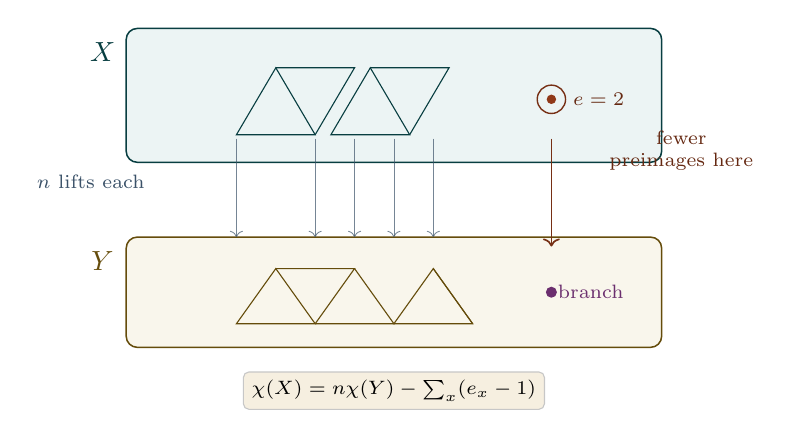
\begin{tikzpicture}[scale=1.0, every node/.style={font=\scriptsize}]
% Top: X with triangulation (n=2 sheets, one ramification)
\begin{scope}[yshift=2.1cm]
  \filldraw[draw=formteal!55!black, fill=formteal!8, line width=0.55pt, rounded corners=4pt]
    (-3.4,-0.85) rectangle (3.4,0.85);
  \node[formteal!55!black, font=\bfseries] at (-3.7,0.55) {$X$};
  % Triangulation: two layers of triangles
  \foreach \xs in {0,1}{
    \begin{scope}[xshift=\xs*1.2cm-2.0cm]
      \draw[formteal!55!black, line width=0.4pt] (0,-0.5) -- (1.0,-0.5) -- (0.5,0.35) -- cycle;
    \end{scope}
    \begin{scope}[xshift=\xs*1.2cm-2.0cm, yshift=0pt]
      \draw[formteal!55!black, line width=0.4pt] (0.5,0.35) -- (1.5,0.35) -- (1.0,-0.5);
    \end{scope}
  }
  % Mark a ramified preimage
  \fill[formrust!85!black] (2.0,-0.05) circle (0.06);
  \draw[formrust!70!black, line width=0.5pt] (2.0,-0.05) circle (0.18);
  \node[formrust!60!black, font=\scriptsize] at (2.6,-0.05) {$e=2$};
\end{scope}
% Bottom: Y with triangulation
\begin{scope}[yshift=-0.4cm]
  \filldraw[draw=formgold!55!black, fill=formgold!8, line width=0.55pt, rounded corners=4pt]
    (-3.4,-0.7) rectangle (3.4,0.7);
  \node[formgold!55!black, font=\bfseries] at (-3.7,0.4) {$Y$};
  % Single triangulation row
  \draw[formgold!55!black, line width=0.4pt] (-2.0,-0.4) -- (-1.0,-0.4) -- (-1.5,0.3) -- cycle;
  \draw[formgold!55!black, line width=0.4pt] (-1.5,0.3) -- (-0.5,0.3) -- (-1.0,-0.4);
  \draw[formgold!55!black, line width=0.4pt] (-0.5,0.3) -- (0.0,-0.4) -- (-1.0,-0.4);
  \draw[formgold!55!black, line width=0.4pt] (0.0,-0.4) -- (1.0,-0.4) -- (0.5,0.3) -- cycle;
  \draw[formgold!55!black, line width=0.4pt] (0.5,0.3) -- (1.0,-0.4);
  % Branch value at one vertex
  \fill[formplum] (2.0,0.0) circle (0.07);
  \node[formplum, font=\scriptsize] at (2.5,0.0) {branch};
\end{scope}
% Arrows showing lifts
\foreach \xx in {-2.0,-1.0,-0.5,0.0,0.5}{
  \draw[->, formslate, line width=0.3pt, opacity=0.7] (\xx,1.55) -- (\xx,0.3);
}
% Vertex correction at ramification
\draw[->, formrust!70!black, line width=0.6pt] (2.0,1.55) -- (2.0,0.18);
\node[formslate, font=\scriptsize] at (-3.85,1.0) {$n$ lifts each};
\node[formrust!60!black, font=\scriptsize, align=center] at (3.65,1.4) {fewer\\preimages here};
% Caption
\node[font=\scriptsize, align=center, fill=formivory, rounded corners=2pt, inner sep=3pt, draw=black!22]
  at (0,-1.65) {$\chi(X)=n\chi(Y)-\sum_x(e_x-1)$};
\end{tikzpicture}
\visualcaption{A triangulation of $Y$ with branch values among the vertices lifts to a triangulation of $X$ in which every edge and face gets $n=\deg f$ copies but the vertex count loses $\sum_x(e_x-1)$ due to ramification. The Euler characteristic carries the correction.}
\end{center}

\section*{Problem 12: Degree of a Canonical Divisor}

\begin{intentrequirements}
\item \textbf{Intent.} Use Riemann--Hurwitz to prove the degree of any canonical divisor on a compact Riemann surface:
\[
 \deg K=2g-2=-\chi(M).
\]
\item \textbf{Required outputs.} Choose a nonconstant meromorphic function $f:M\to\CP^1$, compute $\deg(df)$ from ramification and poles over $\infty$, use Riemann--Hurwitz to identify that degree with $-\chi(M)$, and show all meromorphic $1$-forms have the same divisor degree.
\item \textbf{Required explanations.} Distinguish the local computations at finite target values and at points over $\infty$:
\[
 f=z^e \Rightarrow \ord(df)=e-1,\qquad
 f=z^{-e}\Rightarrow \ord(df)=-(e+1).
\]
\item \textbf{Common pitfalls to avoid.} Do not prove the formula only for $df$. To handle an arbitrary meromorphic $1$-form $\omega$, use $\omega=h\,df$ and the fact that principal divisors have degree zero.
\end{intentrequirements}

\windingnote{The formula $\deg K=2g-2=-\chi(M)$ ties the canonical-divisor degree to the topological winding count of the surface. On $\CP^1$ (genus $0$), $\deg K=-2$: $dz$ has a double pole at $\infty$ because traversing the equator clockwise from above means going counterclockwise from below; the winding form goes around \emph{twice} in the change of coordinates $w=1/z$. On the torus ($g=1$), $\deg K=0$ because $dz$ descends to a nowhere-vanishing holomorphic $1$-form --- there is no winding obstruction. On a higher genus surface ($g\geq 2$), every meromorphic $1$-form has positive total order $2g-2$, reflecting accumulated topological complexity. The whole formula is a global Riemann--Hurwitz residue identity for $df/f$ (Problem~9 plus Problem~11).}

\handsketch{%
\fill[handpaper] (-3.4,-1.9) rectangle (3.4,1.9);
\draw[hand] (-3.4,-1.9) rectangle (3.4,1.9);
% Three surfaces side by side
\begin{scope}[xshift=-2.1cm]
  \draw[handthick] (0,0) circle (0.6);
  \draw[draw=handink, line width=0.4pt, opacity=0.5] (0,0) ellipse (0.6 and 0.2);
  \node[handnote] at (0,-0.95) {$g=0$};
  \node[handnote] at (0,-1.3) {$\deg K=-2$};
\end{scope}
\begin{scope}
  \draw[handthick] (0,0) ellipse (0.8 and 0.42);
  \fill[white] (0,0) ellipse (0.35 and 0.13);
  \draw[draw=handink, line width=0.55pt] (0,0) ellipse (0.35 and 0.13);
  \node[handnote] at (0,-0.95) {$g=1$};
  \node[handnote] at (0,-1.3) {$\deg K=0$};
\end{scope}
\begin{scope}[xshift=2.1cm]
  \draw[handthick] plot[smooth cycle] coordinates {(-0.95,-0.3) (-0.85,0.3) (-0.2,0.4) (0.3,0.3) (0.85,0.4) (0.95,-0.3) (0.4,-0.5) (-0.4,-0.5)};
  \fill[white] (-0.45,0.05) ellipse (0.18 and 0.06);
  \draw[draw=handink, line width=0.45pt] (-0.45,0.05) ellipse (0.18 and 0.06);
  \fill[white] (0.45,0.05) ellipse (0.18 and 0.06);
  \draw[draw=handink, line width=0.45pt] (0.45,0.05) ellipse (0.18 and 0.06);
  \node[handnote] at (0,-0.95) {$g=2$};
  \node[handnote] at (0,-1.3) {$\deg K=+2$};
\end{scope}
\node[handnote] at (0,1.55) {$\deg K=2g-2=-\chi$};
\node[handnote] at (0,-1.85) {arithmetic progression $-2,0,+2,\dots$};
}

Let $M$ be compact and let $\omega$ be a nonzero meromorphic $1$-form. We prove
\[
 \deg(\omega)=-\chi(M).
\]
Since $\chi(M)=2-2g$, this is the familiar formula
\[
 \deg(\omega)=2g-2.
\]

Choose a nonconstant meromorphic function
\[
 f:M\to\CP^1.
\]
Then $df$ is a nonzero meromorphic $1$-form. Let $n=\deg f$ and let
\[
 R=\sum_{p\in M}(e_p(f)-1)
\]
be the total ramification.

We compute the divisor degree of $df$. If $f(p)\neq\infty$, then in a local coordinate one can write
\[
 f(z)-f(p)=z^{e_p}.
\]
Thus
\[
 df=e_pz^{e_p-1}\,dz,
\]
so
\[
 \ord_p(df)=e_p-1.
\]
If $f(p)=\infty$, write $w=1/f$. Locally $w=z^{e_p}$, so
\[
 f=z^{-e_p},\qquad df=-e_p z^{-e_p-1}\,dz.
\]
Thus
\[
 \ord_p(df)=-(e_p+1)=(e_p-1)-2e_p.
\]
Therefore
\[
 \deg(df)
 =
 \sum_{p\in M}(e_p-1)-2\sum_{p\in f^{-1}(\infty)}e_p
 =
 R-2n.
\]
By Riemann-Hurwitz for $f:M\to\CP^1$,
\[
 \chi(M)=2n-R.
\]
Hence
\[
 \deg(df)=R-2n=-\chi(M).
\]

Finally, any two nonzero meromorphic $1$-forms differ by a nonzero meromorphic function. Thus
\[
 \omega=h\,df
\]
for some meromorphic function $h$. Then
\[
 (\omega)=(h)+(df).
\]
The degree of a principal divisor is zero by Problem 9, so
\[
 \deg(\omega)=\deg(df)=-\chi(M).
\]

\begin{center}
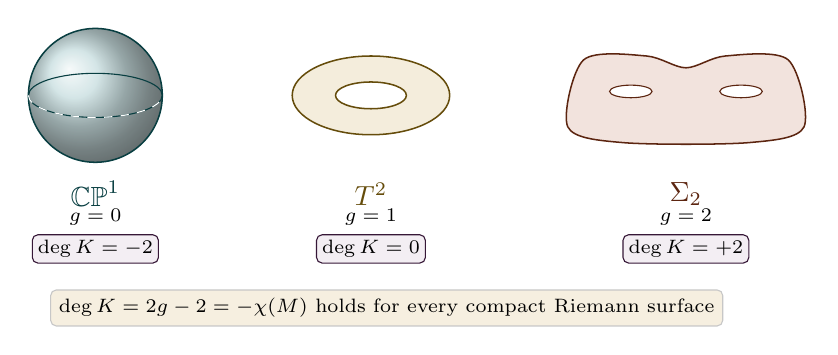
\begin{tikzpicture}[scale=1.0, every node/.style={font=\scriptsize}]
% Three surfaces of increasing genus
% Genus 0: sphere
\begin{scope}
  \shade[ball color=formteal!28, opacity=0.85] (0,0) circle (0.85);
  \draw[formteal!55!black, line width=0.55pt] (0,0) circle (0.85);
  \draw[formteal!55!black, line width=0.4pt] (0,0) ellipse (0.85 and 0.28);
  \draw[dashed, white, line width=0.4pt] (-0.85,0) arc (180:360:0.85 and 0.28);
  \node[formteal!55!black, font=\bfseries] at (0,-1.25) {$\CP^1$};
  \node[font=\scriptsize] at (0,-1.55) {$g=0$};
  \node[draw=formplum!50!black, fill=formplum!8, rounded corners=2pt, font=\scriptsize,
        inner sep=2pt, line width=0.4pt] at (0,-1.95) {$\deg K=-2$};
\end{scope}
% Genus 1: torus
\begin{scope}[xshift=3.5cm]
  \filldraw[draw=formgold!55!black, fill=formgold!15, line width=0.55pt] (0,0) ellipse (1.0 and 0.5);
  \fill[white] (0,0) ellipse (0.45 and 0.17);
  \draw[formgold!55!black, line width=0.55pt] (0,0) ellipse (0.45 and 0.17);
  \node[formgold!55!black, font=\bfseries] at (0,-1.25) {$T^2$};
  \node[font=\scriptsize] at (0,-1.55) {$g=1$};
  \node[draw=formplum!50!black, fill=formplum!8, rounded corners=2pt, font=\scriptsize,
        inner sep=2pt, line width=0.4pt] at (0,-1.95) {$\deg K=0$};
\end{scope}
% Genus 2: two-handled surface
\begin{scope}[xshift=7.5cm]
  \filldraw[draw=formrust!55!black, fill=formrust!15, line width=0.55pt]
    plot[smooth cycle] coordinates {(-1.5,-0.4) (-1.3,0.45) (-0.5,0.5) (0,0.35) (0.5,0.5) (1.3,0.45) (1.5,-0.4) (0.8,-0.6) (-0.8,-0.6)};
  \fill[white] (-0.7,0.05) ellipse (0.27 and 0.08);
  \draw[formrust!55!black, line width=0.4pt] (-0.7,0.05) ellipse (0.27 and 0.08);
  \fill[white] (0.7,0.05) ellipse (0.27 and 0.08);
  \draw[formrust!55!black, line width=0.4pt] (0.7,0.05) ellipse (0.27 and 0.08);
  \node[formrust!55!black, font=\bfseries] at (0,-1.25) {$\Sigma_2$};
  \node[font=\scriptsize] at (0,-1.55) {$g=2$};
  \node[draw=formplum!50!black, fill=formplum!8, rounded corners=2pt, font=\scriptsize,
        inner sep=2pt, line width=0.4pt] at (0,-1.95) {$\deg K=+2$};
\end{scope}
% Bottom equation
\node[font=\scriptsize, align=center, fill=formivory, rounded corners=2pt, inner sep=3pt, draw=black!22]
  at (3.7,-2.7) {$\deg K=2g-2=-\chi(M)$ holds for every compact Riemann surface};
\end{tikzpicture}
\visualcaption{The degree of a canonical divisor rises with the genus in arithmetic progression $-2,0,+2,\ldots$, exactly mirroring the drop of the Euler characteristic. Riemann--Hurwitz shows this is invariant: every meromorphic $1$-form on a fixed surface has the same divisor degree.}
\end{center}

\section*{Problem 13: The Spaces $L(D)$, $I(D)$, and the Case $L(p)$}

\begin{intentrequirements}
\item \textbf{Intent.} Relate meromorphic functions and meromorphic differentials via a chosen canonical divisor, and use this relation to bound $\ell(p)$.
\item \textbf{Required outputs.} Prove the natural isomorphisms
\[
 I(K-D)\cong L(D),\qquad I(D)\cong L(K-D),
\]
and prove $\ell(p)\leq2$ for every point $p$.
\item \textbf{Required explanations.} Choose a meromorphic $1$-form $\eta$ with $(\eta)=K$ and show multiplication or division by $\eta$ converts the divisor inequalities exactly.
\item \textbf{Common pitfalls to avoid.} In the proof of $\ell(p)\leq2$, a nonconstant function in $L(p)$ has at most one simple pole, hence defines a degree-one map to $\CP^1$. This is the key geometric input.
\end{intentrequirements}

\windingnote{The duality $L(D)\cong I(K-D)$ and $I(D)\cong L(K-D)$ is the algebraic shadow of Serre duality, which in turn is built on the residue pairing. For $f\in L(D)$ and $\omega\in I(K-D)$, the pairing $(f,\omega)\mapsto\sum_p\Res_p(f\omega)$ vanishes \emph{globally} on a compact Riemann surface (by Problem~8), exposing $L(D)$ and $I(K-D)$ as dual vector spaces via this residue. The residue here is the same winding-form integral as before --- one is integrating $f\omega$ around each pole and accumulating $1/(2\pi i)$ times the winding integral. The Riemann--Roch theorem (Problems 14--16) is the dimension-theoretic shadow of this pairing.}

\handsketch{%
\fill[handpaper] (-3.4,-1.9) rectangle (3.4,1.9);
\draw[hand] (-3.4,-1.9) rectangle (3.4,1.9);
% L(D) box
\draw[handthick, fill=handink!8] (-2.7,0.6) rectangle (-0.5,1.5);
\node[handnote] at (-1.6,1.05) {$f\in L(D)$};
% I(K-D) box
\draw[handthick, fill=handsepia!10] (0.5,0.6) rectangle (2.7,1.5);
\node[handnote] at (1.6,1.05) {$\omega\in I(K-D)$};
% Pairing arrow
\draw[draw=handink, line width=0.7pt, -{Latex[length=2.0mm]}] (-0.5,1.05) -- (0.5,1.05);
\node[handnote] at (0,1.25) {$f\omega$};
\node[handnote] at (0,0.78) {meromorphic};
% Down arrow to residue
\draw[draw=handink, line width=0.7pt, -{Latex[length=2.0mm]}] (0,0.55) -- (0,-0.05);
\node[handnote] at (0.45,0.25) {residue};
% Center: residue pairing
\draw[handthick, fill=handink!8] (-1.5,-0.85) rectangle (1.5,-0.05);
\node[handnote] at (0,-0.45) {$\displaystyle\sum_p \mathrm{Res}_p(f\omega)=0$};
\node[handnote] at (0,-1.2) {residue pairing};
\node[handnote] at (0,-1.65) {$L(D)\cong I(K-D)^{\vee}$ (Serre duality)};
}

Throughout Problem 13, let $K$ be a canonical divisor on $X$, and choose a nonzero meromorphic $1$-form $\eta$ with
\[
 K=(\eta).
\]

\subsection*{Problem 13-1: The isomorphism $I(K-D)\cong L(D)$}

Define
\[
 L(D)\longrightarrow I(K-D),\qquad f\longmapsto f\eta.
\]
This map is linear. Moreover,
\[
 (f\eta)-(K-D)
 =
 (f)+(\eta)-K+D
 =
 (f)+D,
\]
using $(\eta)=K$. Therefore $f\eta\in I(K-D)$ if and only if $(f\eta)-(K-D)\geq 0$, which is the same as $(f)+D\geq 0$, i.e.\ $f\in L(D)$. The inverse map
\[
 I(K-D)\longrightarrow L(D),\qquad \omega\longmapsto \frac{\omega}{\eta},
\]
is the same construction in reverse. Hence
\[
 I(K-D)\cong L(D).
\]

\subsection*{Problem 13-2: The isomorphism $I(D)\cong L(K-D)$}

Similarly, define
\[
 I(D)\longrightarrow L(K-D),\qquad \omega\longmapsto \frac{\omega}{\eta}.
\]
For the divisor calculation,
\[
 \left(\frac{\omega}{\eta}\right)+(K-D)
 =
 (\omega)-(\eta)+K-D
 =
 (\omega)-D,
\]
again using $(\eta)=K$. Hence $\omega/\eta\in L(K-D)$ if and only if $(\omega)-D\geq 0$, i.e.\ $\omega\in I(D)$. The inverse is multiplication by $\eta$. Therefore
\[
 I(D)\cong L(K-D).
\]

\subsection*{Problem 13-3: The estimate $\ell(p)\leq 2$}

Constants always give a one-dimensional subspace of $L(p)$, so $\ell(p)\geq 1$. If $L(p)$ contains no nonconstant function, then $\ell(p)=1\leq 2$ and we are done.

Suppose $L(p)$ contains a nonconstant function $f$. Since a holomorphic function on a compact Riemann surface is constant, $f$ must have a pole. The condition $f\in L(p)$ says that the only possible pole is a simple pole at $p$. Hence, as a map
\[
 f:X\to\CP^1,
\]
the fiber over $\infty$ consists of the single point $p$ with multiplicity $1$, so $\deg f=1$.

A degree-one holomorphic map between compact Riemann surfaces is biholomorphic: every fiber consists of one unramified point, so the map is bijective and locally biholomorphic. Thus $X\cong\CP^1$.

On $\CP^1$, after moving $p$ to $\infty$, the meromorphic functions with at most a simple pole at $p$ are exactly the polynomials of degree at most $1$:
\[
 f(z)=a+bz,\qquad a,b\in\C.
\]
This space has dimension $2$. Therefore in all cases
\[
 \ell(p)\leq 2,
\]
with equality if and only if $X\cong\CP^1$.

\begin{center}
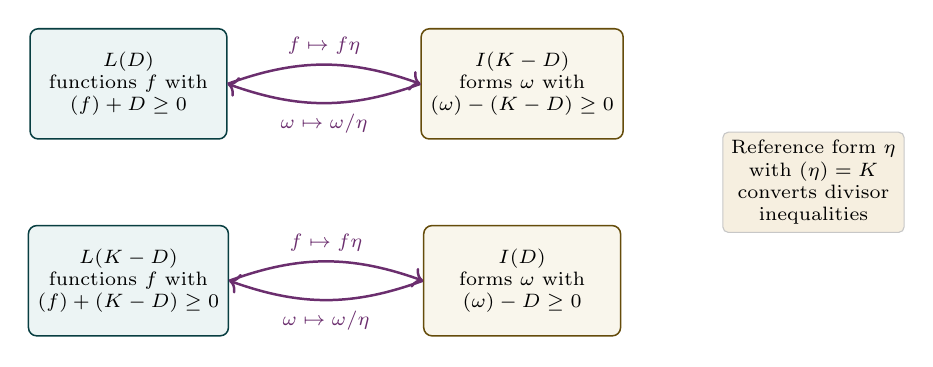
\begin{tikzpicture}[scale=1.0, every node/.style={font=\scriptsize}]
% L(D) box
\node[draw=formteal!55!black, fill=formteal!8, line width=0.55pt, rounded corners=3pt,
      align=center, minimum width=2.5cm, minimum height=1.4cm] (LD) at (0,0)
      {$L(D)$\\\scriptsize functions $f$ with\\$(f)+D\geq 0$};
% I(K-D) box
\node[draw=formgold!55!black, fill=formgold!8, line width=0.55pt, rounded corners=3pt,
      align=center, minimum width=2.5cm, minimum height=1.4cm] (IKD) at (5.0,0)
      {$I(K-D)$\\\scriptsize forms $\omega$ with\\$(\omega)-(K-D)\geq 0$};
% Arrows: multiplication and division
\draw[->, formplum, line width=0.9pt] (LD.east) to[bend left=20] node[midway, above, formplum] {$f\mapsto f\eta$} (IKD.west);
\draw[->, formplum, line width=0.9pt] (IKD.west) to[bend left=20] node[midway, below, formplum] {$\omega\mapsto\omega/\eta$} (LD.east);
% L(K-D) box
\node[draw=formteal!55!black, fill=formteal!8, line width=0.55pt, rounded corners=3pt,
      align=center, minimum width=2.5cm, minimum height=1.4cm] (LKD) at (0,-2.5)
      {$L(K-D)$\\\scriptsize functions $f$ with\\$(f)+(K-D)\geq 0$};
\node[draw=formgold!55!black, fill=formgold!8, line width=0.55pt, rounded corners=3pt,
      align=center, minimum width=2.5cm, minimum height=1.4cm] (ID) at (5.0,-2.5)
      {$I(D)$\\\scriptsize forms $\omega$ with\\$(\omega)-D\geq 0$};
\draw[->, formplum, line width=0.9pt] (LKD.east) to[bend left=20] node[midway, above, formplum] {$f\mapsto f\eta$} (ID.west);
\draw[->, formplum, line width=0.9pt] (ID.west) to[bend left=20] node[midway, below, formplum] {$\omega\mapsto\omega/\eta$} (LKD.east);
% Diagonal/Serre annotation
\node[font=\scriptsize, align=center, fill=formivory, rounded corners=2pt, inner sep=3pt, draw=black!22]
  at (8.7,-1.25) {Reference form $\eta$\\with $(\eta)=K$\\converts divisor\\inequalities};
\end{tikzpicture}
\visualcaption{A choice of nonzero meromorphic $1$-form $\eta$ with $(\eta)=K$ produces natural isomorphisms between function spaces and form spaces, swapping $D$ with $K-D$. This is the algebraic engine behind Serre duality and the symmetry of Riemann--Roch.}
\end{center}

\section*{Problem 14: Riemann-Roch, Step 1}

\begin{intentrequirements}
\item \textbf{Intent.} Prove Riemann--Roch first for effective divisors using the principal-parts criterion and residue pairings with holomorphic differentials.
\item \textbf{Required outputs.} State the principal-parts criterion and prove that for $D\geq0$,
\[
 \ell(D)-i(D)=\deg D+1-g.
\]
\item \textbf{Required explanations.} Count the vector space of possible principal parts, identify the kernel of the principal-part map as constants, and show that the annihilator of all allowed principal parts is exactly $I(D)$.
\item \textbf{Common pitfalls to avoid.} The dimension of holomorphic $1$-forms is $g$, and the obstruction rank is $g-i(D)$, not simply $g$.
\end{intentrequirements}

\windingnote{The principal-parts criterion is the residue theorem applied to test forms. A prescribed principal part $P_j(z_j)=\sum_{k=1}^{m_j}c_{j,k}z_j^{-k}$ at $a_j$ can be realized by a global meromorphic function $f\in L(D)$ if and only if, for every holomorphic $1$-form $\omega$, the residue sum $\sum_j\Res_{a_j}(P_j\omega)$ vanishes. Each summand $\Res_{a_j}(P_j\omega)$ is a winding-form integral $\frac{1}{2\pi i}\oint_\gamma P_j\omega$, and the vanishing of the total is forced by Problem~8 because, if $f$ exists, then $f\omega$ is a meromorphic $1$-form whose residues at the $a_j$ are exactly these residues plus contributions from poles of $\omega$ (which cancel because $\omega$ is holomorphic). So Riemann--Roch's count uses the winding-form residue pairing as its only nontrivial constraint.}

\handsketch{%
\fill[handpaper] (-3.4,-1.9) rectangle (3.4,1.9);
\draw[hand] (-3.4,-1.9) rectangle (3.4,1.9);
% Surface with three poles
\draw[handthick] plot[smooth cycle] coordinates {(-2.8,-0.6) (-2.4,0.6) (-0.8,0.85) (0.8,0.7) (2.4,0.6) (2.8,-0.6) (1.0,-1.0) (-1.0,-1.0)};
% Three points a1, a2, a3 with prescribed principal parts
\foreach \xx/\yy/\lbl/\pp in {-1.8/0.25/$a_1$/$P_1=c_{1}/z_1$, 0/0.45/$a_2$/$P_2=c_{2}/z_2^2$, 1.6/-0.05/$a_3$/$P_3=c_{3}/z_3$}{
  \fill[handink] (\xx,\yy) circle (0.06);
  \draw[draw=handink, line width=0.55pt] (\xx,\yy) circle (0.18);
  \node[handnote] at (\xx,\yy-0.4) {\lbl};
}
\node[handnote] at (-1.8,0.85) {$P_1$};
\node[handnote] at (0,1.05) {$P_2$};
\node[handnote] at (1.6,0.55) {$P_3$};
\node[handnote] at (0,-1.4) {$\Sigma_j\,\mathrm{Res}_{a_j}(P_j\omega)=0\;\;\forall\omega\in H^0(K)$};
\node[handnote] at (0,-1.85) {$\Leftrightarrow$ realizable as $f\in L(D)$};
}

Let $X$ have genus $g$, and let $D\geq0$ be effective:
\[
 D=\sum_{j=1}^n m_j a_j,
\qquad m_j\geq1.
\]

\subsection*{Principal-parts criterion}

Given principal parts $P_j$ at the points $a_j$, there exists a meromorphic function on $X$ with those principal parts and no other poles if and only if for every holomorphic $1$-form $\omega$ on $X$,
\[
 \sum_{j=1}^n \Res_{a_j}(P_j\omega)=0.
\]

\subsection*{Proof of the formula for effective $D$}

Let $V$ be the vector space of possible principal parts bounded by $D$:
\[
 P_j(z_j)=\sum_{k=1}^{m_j}c_{j,k}z_j^{-k}
\]
at each $a_j$. Then
\[
 \dim_\C V=\sum_{j=1}^n m_j=\deg D.
\]
There is a linear map
\[
 L(D)\to V
\]
sending a meromorphic function to its collection of principal parts at the $a_j$'s. The kernel consists of holomorphic functions on compact $X$, hence constants. Therefore
\[
 \dim(\operatorname{image})=\ell(D)-1.
\]

By the principal-parts criterion, the image is the kernel of
\[
 \Phi:V\to H^0(X,K)^*,
 \qquad
 P\mapsto\left(\omega\mapsto\sum_j\Res_{a_j}(P_j\omega)\right).
\]
We compute the rank of $\Phi$ by computing the kernel of the dual map. A holomorphic $1$-form $\omega$ lies in the kernel of the dual map exactly when
\[
 \Res_{a_j}(P_j\omega)=0
\]
for every allowed principal part $P_j$ at every $a_j$.
In a coordinate $z_j$, write
\[
 \omega=h_j(z_j)\,dz_j.
\]
Taking $P_j=z_j^{-k}$ shows that the residue is the coefficient of $z_j^{k-1}$ in $h_j$. Thus all these residues vanish for $k=1,\dots,m_j$ exactly when
\[
 \ord_{a_j}(\omega)\geq m_j.
\]
Hence the kernel is precisely $I(D)$, whose dimension is $i(D)$.

Since
\[
 \dim H^0(X,K)=g,
\]
we get
\[
 \operatorname{rank}\Phi=g-i(D).
\]
Therefore
\[
 \ell(D)-1
 =
 \dim\ker\Phi
 =
 \deg D-(g-i(D)).
\]
Rearranging gives
\[
 \boxed{\ell(D)-i(D)=\deg D+1-g.}
\]

\begin{center}
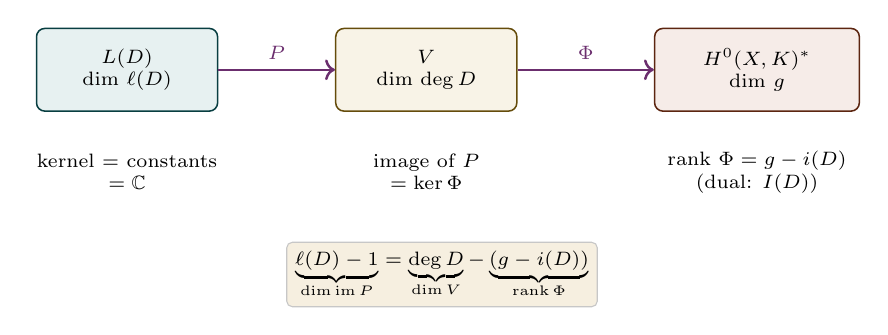
\begin{tikzpicture}[scale=1.0, every node/.style={font=\scriptsize}]
% L(D) (largest)
\node[draw=formteal!55!black, fill=formteal!10, line width=0.55pt, rounded corners=3pt,
      align=center, minimum width=2.3cm, minimum height=1.05cm] (LD) at (0,0)
      {$L(D)$\\dim $\ell(D)$};
% V (principal parts)
\node[draw=formgold!55!black, fill=formgold!10, line width=0.55pt, rounded corners=3pt,
      align=center, minimum width=2.3cm, minimum height=1.05cm] (V) at (3.8,0)
      {$V$\\dim $\deg D$};
% Residue dual
\node[draw=formrust!55!black, fill=formrust!10, line width=0.55pt, rounded corners=3pt,
      align=center, minimum width=2.6cm, minimum height=1.05cm] (H) at (8.0,0)
      {$H^0(X,K)^*$\\dim $g$};
% Maps
\draw[->, formplum, line width=0.9pt] (LD.east) -- node[midway, above, formplum] {$P$} (V.west);
\draw[->, formplum, line width=0.9pt] (V.east) -- node[midway, above, formplum] {$\Phi$} (H.west);
% Below: kernel/cokernel info
\node[font=\scriptsize, align=center] at (0,-1.3) {kernel $=$ constants\\$=\C$};
\node[font=\scriptsize, align=center] at (3.8,-1.3) {image of $P$\\$=\ker\Phi$};
\node[font=\scriptsize, align=center] at (8.0,-1.3) {rank $\Phi=g-i(D)$\\(dual: $I(D)$)};
% Dimension equation
\node[font=\scriptsize, fill=formivory, rounded corners=2pt, inner sep=3pt, draw=black!22]
  at (4.0,-2.6) {$\underbrace{\ell(D)-1}_{\dim\im P} =\underbrace{\deg D}_{\dim V}-\underbrace{(g-i(D))}_{\operatorname{rank}\Phi}$};
\end{tikzpicture}
\visualcaption{The Riemann--Roch dimension count threads through a single linear sequence: functions $\to$ principal parts $\to$ residue pairing with holomorphic differentials. The kernel-and-rank arithmetic on this sequence is exactly the Riemann--Roch formula for effective divisors.}
\end{center}

\section*{Problem 15: Riemann-Roch, Step 2}

\begin{intentrequirements}
\item \textbf{Intent.} Extend the effective-divisor Riemann--Roch result to a one-sided inequality for arbitrary divisors by subtracting points one at a time.
\item \textbf{Required outputs.} Prove
\[
 \ell(D)-i(D)\geq\deg D+1-g
\]
for every divisor $D$.
\item \textbf{Required explanations.} Compare $D$ and $D-a$, show that $\ell$ can drop by at most one and $i$ can rise by at most one, and prove that both jumps cannot occur simultaneously using the residue theorem.
\item \textbf{Common pitfalls to avoid.} The contradiction uses a meromorphic $1$-form with exactly one simple pole and nonzero residue. This is impossible on a compact Riemann surface.
\end{intentrequirements}

We prove that for every divisor $D$,
\[
 \ell(D)-i(D)\geq \deg D+1-g.
\]

Define
\[
 R(D)=\ell(D)-i(D)-\deg D-1+g.
\]
Problem 14 says that
\[
 R(D)=0
\]
whenever $D\geq0$.

Now compare $D$ and $D-a$ for a point $a\in X$. Since
\[
 L(D-a)\subset L(D),
\]
the quotient has dimension at most $1$, so
\[
 \ell(D-a)=\ell(D)\quad\text{or}\quad \ell(D)-1.
\]
Similarly,
\[
 I(D)\subset I(D-a),
\]
and
\[
 i(D-a)=i(D)\quad\text{or}\quad i(D)+1.
\]

We claim the two jumps
\[
 \ell(D-a)=\ell(D)-1
 \quad\text{and}\quad
 i(D-a)=i(D)+1
\]
cannot occur simultaneously.
If they did, there would be
\[
 f\in L(D)\setminus L(D-a)
\]
and
\[
 \omega\in I(D-a)\setminus I(D).
\]
Let the coefficient of $D$ at $a$ be $n$. Then locally
\[
 \ord_a(f)=-n,\qquad \ord_a(\omega)=n-1.
\]
Therefore $f\omega$ has a simple pole at $a$ with nonzero residue. At every other point $q\neq a$, the inequalities defining $L(D)$ and $I(D-a)$ imply that $f\omega$ is holomorphic. Thus $f\omega$ would be a meromorphic $1$-form on compact $X$ with exactly one pole and nonzero residue. This contradicts the residue theorem, since the sum of all residues must be zero.

Thus the two jumps cannot both happen. If
\[
 \alpha=\ell(D)-\ell(D-a),\qquad
 \beta=i(D-a)-i(D),
\]
then $\alpha,\beta\in\{0,1\}$ and $\alpha+\beta\leq1$. Hence
\[
\begin{aligned}
 R(D-a)
 &=\ell(D-a)-i(D-a)-\deg(D-a)-1+g\\
 &=R(D)+1-\alpha-\beta\\
 &\geq R(D).
\end{aligned}
\]

Starting from a sufficiently large effective divisor $E\geq D$, for which $R(E)=0$, and subtracting points one at a time until reaching $D$, we obtain
\[
 R(D)\geq0.
\]
Therefore
\[
 \ell(D)-i(D)\geq\deg D+1-g.
\]

\begin{center}
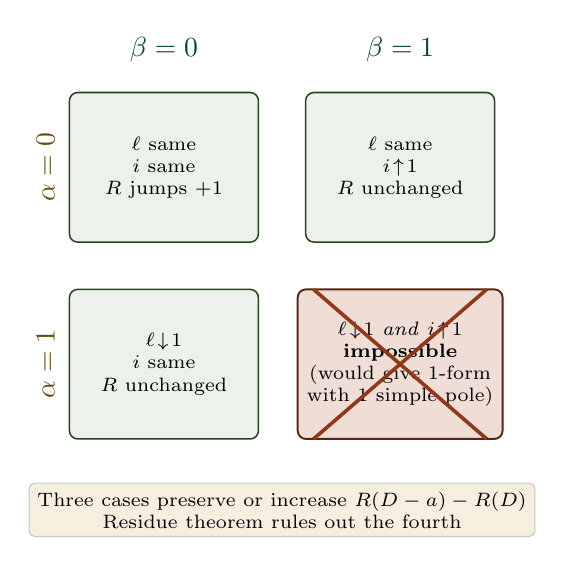
\begin{tikzpicture}[scale=1.0, every node/.style={font=\scriptsize}]
% 2x2 grid of (alpha, beta) possibilities
\node[font=\bfseries, formteal!55!black] at (-1.5,3.0) {$\beta=0$};
\node[font=\bfseries, formteal!55!black] at (1.5,3.0) {$\beta=1$};
\node[font=\bfseries, formgold!55!black, rotate=90] at (-3.0,1.5) {$\alpha=0$};
\node[font=\bfseries, formgold!55!black, rotate=90] at (-3.0,-1.0) {$\alpha=1$};
% (0,0) cell: ℓ and i both unchanged — R increases by 1
\node[draw=formsage!55!black, fill=formsage!10, rounded corners=3pt, line width=0.55pt,
      minimum width=2.4cm, minimum height=1.9cm, align=center] at (-1.5,1.5)
      {$\ell$ same\\$i$ same\\$R$ jumps $+1$};
% (1,0) cell: ℓ drops by 1, i unchanged — R unchanged
\node[draw=formsage!55!black, fill=formsage!10, rounded corners=3pt, line width=0.55pt,
      minimum width=2.4cm, minimum height=1.9cm, align=center] at (1.5,1.5)
      {$\ell$ same\\$i\!\uparrow\!1$\\$R$ unchanged};
% (0,1) cell: ℓ same, i jumps — R unchanged
\node[draw=formsage!55!black, fill=formsage!10, rounded corners=3pt, line width=0.55pt,
      minimum width=2.4cm, minimum height=1.9cm, align=center] at (-1.5,-1.0)
      {$\ell\!\downarrow\!1$\\$i$ same\\$R$ unchanged};
% (1,1) cell: FORBIDDEN
\node[draw=formrust!55!black, fill=formrust!18, rounded corners=3pt, line width=0.7pt,
      minimum width=2.4cm, minimum height=1.9cm, align=center] at (1.5,-1.0)
      {$\ell\!\downarrow\!1$ \emph{and} $i\!\uparrow\!1$\\\textbf{impossible}\\\scriptsize(would give $1$-form\\with $1$ simple pole)};
% Strike through impossible cell
\draw[formrust!85!black, line width=1.3pt] (0.4,-1.95) -- (2.6,-0.05);
\draw[formrust!85!black, line width=1.3pt] (0.4,-0.05) -- (2.6,-1.95);
% Bottom annotation
\node[font=\scriptsize, fill=formivory, rounded corners=2pt, inner sep=3pt, draw=black!22, align=center]
  at (0,-2.85) {Three cases preserve or increase $R(D-a)-R(D)$\\Residue theorem rules out the fourth};
\end{tikzpicture}
\visualcaption{Subtracting a point can decrement $\ell$ or increment $i$, but never both. The forbidden configuration would yield a meromorphic $1$-form with a single simple pole and nonzero residue — barred by the residue theorem.}
\end{center}

\section*{Problem 16: Riemann-Roch, Step 3 and Final Conclusion}

\begin{intentrequirements}
\item \textbf{Intent.} Use duality with $K-D$ to prove the reverse inequality and finish the Riemann--Roch theorem.
\item \textbf{Required outputs.} Apply the inequality from Problem 15 to $K-D$, use
\[
 \ell(K-D)=i(D),\qquad i(K-D)=\ell(D),
\]
substitute $\deg K=2g-2$, and conclude
\[
 \ell(D)-i(D)=\deg D+1-g.
\]
\item \textbf{Required explanations.} Make clear why applying the already-proved inequality to $K-D$ reverses the desired inequality after multiplying by $-1$.
\item \textbf{Common pitfalls to avoid.} Do not forget to use $\deg(K-D)=\deg K-\deg D$ and $\deg K=2g-2$.
\end{intentrequirements}

Apply the inequality from Problem 15 to the divisor $K-D$:
\[
 \ell(K-D)-i(K-D)\geq \deg(K-D)+1-g.
\]
Using the isomorphisms from Problem 13,
\[
 \ell(K-D)=i(D),
\qquad
 i(K-D)=\ell(D).
\]
Thus
\[
 i(D)-\ell(D)\geq \deg K-\deg D+1-g.
\]
Multiplying by $-1$ gives
\[
 \ell(D)-i(D)\leq \deg D-\deg K-1+g.
\]
By Problem 12,
\[
 \deg K=2g-2.
\]
Therefore
\[
 \ell(D)-i(D)
 \leq
 \deg D-(2g-2)-1+g
 =
 \deg D+1-g.
\]

Problem 15 gives the reverse inequality
\[
 \ell(D)-i(D)\geq \deg D+1-g.
\]
Combining the two inequalities yields the Riemann-Roch theorem:
\[
 \boxed{\ell(D)-i(D)=\deg D+1-g.}
\]

\begin{center}
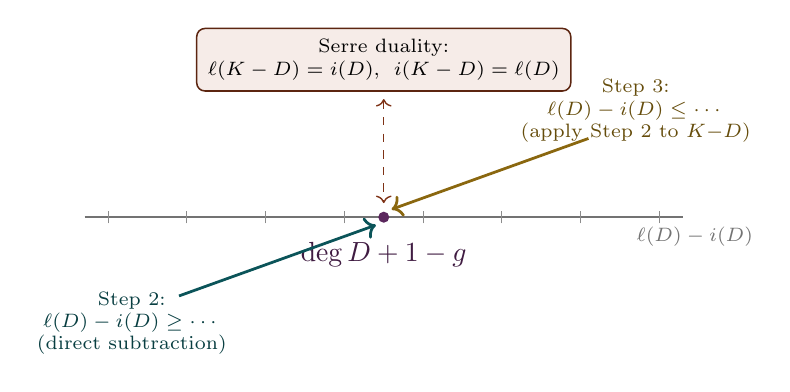
\begin{tikzpicture}[scale=1.0, every node/.style={font=\scriptsize}]
% Number-line axis
\draw[black!55, line width=0.55pt] (-3.8,0) -- (3.8,0);
\foreach \xx in {-3.5,-2.5,-1.5,-0.5,0.5,1.5,2.5,3.5}{
  \draw[black!45, line width=0.35pt] (\xx,-0.08) -- (\xx,0.08);
}
\node[font=\scriptsize, black!55] at (3.95,-0.25) {$\ell(D)-i(D)$};
% The target value
\fill[formplum!85!black] (0,0) circle (0.07);
\node[formplum!60!black, font=\bfseries, below] at (0,-0.2) {$\deg D+1-g$};
% Left-pointing arrow from upper region (the ≤ inequality, from K-D side)
\draw[->, formgold!75!black, line width=1pt] (2.6,1.0) -- (0.1,0.1);
\node[formgold!55!black, font=\scriptsize, align=center] at (3.2,1.35) {Step 3:\\$\ell(D)-i(D)\leq\cdots$\\(apply Step 2 to $K{-}D$)};
% Right-pointing arrow from lower region (the ≥ inequality, from Step 2)
\draw[->, formteal!75!black, line width=1pt] (-2.6,-1.0) -- (-0.1,-0.1);
\node[formteal!55!black, font=\scriptsize, align=center] at (-3.2,-1.35) {Step 2:\\$\ell(D)-i(D)\geq\cdots$\\(direct subtraction)};
% Duality link annotation in the center
\node[draw=formrust!55!black, fill=formrust!10, rounded corners=3pt, font=\scriptsize,
      align=center, inner sep=4pt, line width=0.55pt] at (0,2.0)
      {Serre duality:\\$\ell(K-D)=i(D)$, $\;i(K-D)=\ell(D)$};
\draw[<->, formrust!75!black, line width=0.5pt, dashed] (0,1.5) -- (0,0.18);
\end{tikzpicture}
\visualcaption{Two inequalities pinch the quantity $\ell(D)-i(D)$ from opposite directions: Step 2 supplies the lower bound, and applying the same step to $K-D$ — interpreted through Serre duality — supplies the upper bound. Together they force equality.}
\end{center}

\section*{Problem 17: The Case $\ell(p)\geq2$ and the Sphere}

\begin{intentrequirements}
\item \textbf{Intent.} Characterize the Riemann sphere by the existence of a nonconstant meromorphic function with at most one simple pole.
\item \textbf{Required outputs.} Prove the equivalence of: $X$ is homeomorphic to $S^2$; some $p$ satisfies $\ell(p)\geq2$; and $X$ is biholomorphic to $\CP^1$.
\item \textbf{Required explanations.} Use Riemann--Roch when $g=0$ to get $\ell(p)=2$, and use a nonconstant function in $L(p)$ to build a degree-one holomorphic map $X\to\CP^1$.
\item \textbf{Common pitfalls to avoid.} A degree-one holomorphic map between compact Riemann surfaces is not merely surjective; it is biholomorphic.
\end{intentrequirements}

\windingnote{A nonconstant $f\in L(p)$ has a simple pole at $p$ and is otherwise holomorphic, so $df/f$ has a single simple pole at $p$ with residue $-1$ and a single zero of order $1$ somewhere with residue $+1$ --- summing to $0$ as required by Problem~9. As a map $f:X\to\CP^1$, the winding number around $\infty$ along a small loop near $p$ is $1$; therefore the degree of $f$ is $1$. A degree-one branched cover of compact Riemann surfaces is forced to be unramified everywhere (since the sum of $(e_x-1)$ would have to be $0$ by Riemann--Hurwitz $\chi(X)=\chi(\CP^1)\cdot 1-\sum(e_x-1)$), so $X\cong\CP^1$. Thus the simplest possible winding behavior --- a single simple pole somewhere --- exactly characterizes the Riemann sphere.}

\handsketch{%
\fill[handpaper] (-3.4,-1.9) rectangle (3.4,1.9);
\draw[hand] (-3.4,-1.9) rectangle (3.4,1.9);
% Source X (assumed sphere)
\begin{scope}[xshift=-1.85cm]
  \draw[handthick] (0,0) circle (1.0);
  \draw[draw=handink, line width=0.4pt, opacity=0.5] (0,0) ellipse (1.0 and 0.3);
  \fill[handink] (60:1.0) circle (0.06);
  \node[handnote] at ($(60:1.0)+(60:0.2)$) {$p$};
  \draw[draw=handink, line width=0.55pt] (60:1.0) circle (0.18);
  \node[handnote] at (0,-1.3) {$X$ (genus 0)};
\end{scope}
% Map f: X -> CP^1 with winding 1
\draw[draw=handink, line width=0.8pt, -{Latex[length=2.5mm]}] (-0.75,0) -- (0.55,0);
\node[handnote] at (0,0.3) {$f$, winding 1};
% Target CP^1
\begin{scope}[xshift=1.85cm]
  \draw[handthick] (0,0) circle (1.0);
  \draw[draw=handink, line width=0.4pt, opacity=0.5] (0,0) ellipse (1.0 and 0.3);
  \fill[handink] (60:1.0) circle (0.06);
  \node[handnote] at ($(60:1.0)+(60:0.2)$) {$\infty$};
  \node[handnote] at (0,-1.3) {$\CP^1$};
\end{scope}
\node[handnote] at (0,1.6) {simple pole = degree 1};
\node[handnote] at (0,-1.85) {degree-1 holomorphic $\Rightarrow$ biholomorphic};
}

We prove the equivalence of:
\begin{enumerate}
\item $X$ is homeomorphic to $S^2$.
\item There exists $p\in X$ such that $\ell(p)\geq2$.
\item $X$ is biholomorphic to $\CP^1$.
\end{enumerate}

\textbf{(3) implies (1).}
The Riemann sphere $\CP^1$ is homeomorphic to $S^2$.

\textbf{(1) implies (2).}
If $X$ is homeomorphic to $S^2$, then $g=0$. Apply Riemann-Roch to $D=p$:
\[
 \ell(p)-i(p)=\deg(p)+1-g=2.
\]
Also $i(p)=0$, because a form in $I(p)$ would have divisor at least $p$, hence degree at least $1$, while every canonical divisor has degree
\[
 2g-2=-2.
\]
Thus
\[
 \ell(p)=2.
\]

\textbf{(2) implies (3).}
If $\ell(p)\geq2$, then $L(p)$ contains a nonconstant meromorphic function $f$. Since $f\in L(p)$, its only possible pole is a simple pole at $p$. Since a holomorphic function on compact $X$ is constant, $f$ must have exactly a simple pole at $p$.
Therefore, as a map
\[
 f:X\to\CP^1,
\]
the degree is $1$. A degree-one nonconstant holomorphic map between compact Riemann surfaces is biholomorphic. Hence
\[
 X\cong\CP^1.
\]

\begin{center}
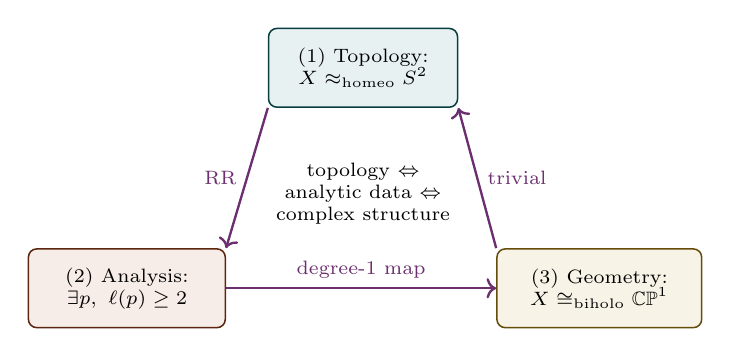
\begin{tikzpicture}[scale=1.0, every node/.style={font=\scriptsize}]
% Three equivalent conditions arranged in triangle
\node[draw=formteal!55!black, fill=formteal!10, line width=0.55pt, rounded corners=3pt,
      align=center, minimum width=2.4cm, minimum height=1.0cm] (top) at (0,2.0)
      {(1) Topology:\\$X\approx_{\text{homeo}}S^2$};
\node[draw=formrust!55!black, fill=formrust!10, line width=0.55pt, rounded corners=3pt,
      align=center, minimum width=2.5cm, minimum height=1.0cm] (left) at (-3.0,-0.8)
      {(2) Analysis:\\$\exists p,\ \ell(p)\geq 2$};
\node[draw=formgold!55!black, fill=formgold!10, line width=0.55pt, rounded corners=3pt,
      align=center, minimum width=2.6cm, minimum height=1.0cm] (right) at (3.0,-0.8)
      {(3) Geometry:\\$X\cong_{\text{biholo}}\CP^1$};
% Arrows
\draw[->, formplum, line width=0.85pt] (top.south west) -- node[midway, left, formplum, font=\scriptsize] {RR} (left.north east);
\draw[->, formplum, line width=0.85pt] (left.east) -- node[midway, above, formplum, font=\scriptsize] {degree-1 map} (right.west);
\draw[->, formplum, line width=0.85pt] (right.north west) -- node[midway, right, formplum, font=\scriptsize] {trivial} (top.south east);
% Center comment
\node[font=\scriptsize, align=center] at (0,0.4) {topology $\Leftrightarrow$\\analytic data $\Leftrightarrow$\\complex structure};
\end{tikzpicture}
\visualcaption{For genus zero the three perspectives coincide: a sphere by topology, the existence of a nonconstant function with a simple pole by Riemann--Roch, and the Riemann sphere as a complex manifold. The proof completes a tight triangle of implications.}
\end{center}

\section*{Problem 18: Asymptotic Riemann-Roch and Base Point Freeness}

\begin{intentrequirements}
\item \textbf{Intent.} Use the large-degree form of Riemann--Roch to prove that sufficiently positive divisors have no base points.
\item \textbf{Required outputs.} State asymptotic Riemann--Roch, prove $i(D)=0$ when $\deg D>2g-2$, and show that if $\deg D\geq2g$, then for each $p$ there is a section in $L(D)$ nonzero at $p$.
\item \textbf{Required explanations.} Compare $\ell(D)$ and $\ell(D-p)$:
\[
 \ell(D)-\ell(D-p)=1.
\]
This strict inequality is the intrinsic base point freeness condition.
\item \textbf{Common pitfalls to avoid.} For arbitrary divisors, ``$f(p)\neq0$'' should be read in the local trivialization of $\mathcal O(D)$, i.e. as nonvanishing of the corresponding section at $p$.
\end{intentrequirements}

\textbf{Asymptotic Riemann-Roch.}
If $D$ is a divisor on a compact Riemann surface of genus $g$ and
\[
 \deg D>2g-2,
\]
then
\[
 i(D)=0
\]
and hence
\[
 \ell(D)=\deg D+1-g.
\]
Indeed, $i(D)=\ell(K-D)$, and
\[
 \deg(K-D)=2g-2-\deg D<0,
\]
so $L(K-D)=0$.

Now assume
\[
 \deg D\geq 2g.
\]
Then for every $p\in X$,
\[
 \deg(D-p)\geq2g-1>2g-2.
\]
Thus asymptotic Riemann-Roch applies to both $D$ and $D-p$:
\[
 \ell(D)=\deg D+1-g,
\]
and
\[
 \ell(D-p)=\deg(D-p)+1-g=\deg D-g.
\]
Therefore
\[
 \ell(D)-\ell(D-p)=1.
\]
So
\[
 L(D-p)\subsetneq L(D).
\]
Choose
\[
 f\in L(D)\setminus L(D-p).
\]
This means that at $p$ the section represented by $f$ does not vanish. In divisor language,
\[
 \ord_p(f)+D_p=0.
\]
In a local trivialization of the line bundle $\mathcal O(D)$, this is exactly the statement that the corresponding section has nonzero value at $p$.
Thus the complete linear system associated to $D$ is base point free.

\emph{Convention note.} If one writes elements of $L(D)$ only as meromorphic functions, the intrinsic base point free condition is $L(D-p)\neq L(D)$ for every $p$. When $D_p=0$, this condition is literally the existence of $f\in L(D)$ with $f(p)\neq0$.

\begin{center}
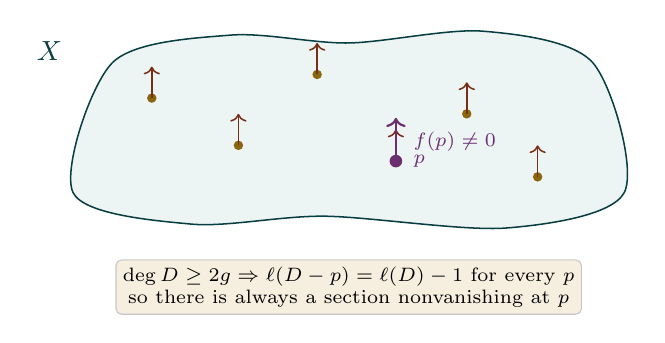
\begin{tikzpicture}[scale=1.0, every node/.style={font=\scriptsize}]
% Riemann surface
\filldraw[draw=formteal!55!black, fill=formteal!8, line width=0.55pt]
  plot[smooth cycle] coordinates {(-3.5,-0.8) (-3.0,0.85) (-1.5,1.2) (0,1.1) (1.7,1.25) (3.1,0.85) (3.5,-0.8) (2.0,-1.25) (-0.3,-1.1) (-2.0,-1.2)};
% Sample points across the surface
\foreach \xx/\yy in {-2.5/0.4, -1.4/-0.2, -0.4/0.7, 0.6/-0.4, 1.5/0.2, 2.4/-0.6}{
  \fill[formgold!75!black] (\xx,\yy) circle (0.06);
}
\node[formteal!55!black, font=\bfseries] at (-3.8,1.0) {$X$};
% Section vectors emanating from each point
\foreach \xx/\yy in {-2.5/0.4, -1.4/-0.2, -0.4/0.7, 0.6/-0.4, 1.5/0.2, 2.4/-0.6}{
  \draw[->, formrust!70!black, line width=0.55pt] (\xx,\yy) -- ++(0.0,0.4);
}
% A picked point p with section nonzero
\fill[formplum] (0.6,-0.4) circle (0.08);
\draw[->, formplum, line width=0.8pt] (0.6,-0.4) -- (0.6,0.15);
\node[formplum, font=\scriptsize, right] at (0.7,-0.4) {$p$};
\node[formplum, font=\scriptsize, right] at (0.7,-0.15) {$f(p)\neq 0$};
% Caption
\node[font=\scriptsize, fill=formivory, rounded corners=2pt, inner sep=2.5pt, draw=black!22, align=center]
  at (0,-2.0) {$\deg D\geq 2g\Rightarrow\ell(D-p)=\ell(D)-1$ for every $p$\\so there is always a section nonvanishing at $p$};
\end{tikzpicture}
\visualcaption{When $\deg D\geq 2g$, the strict drop $\ell(D-p)<\ell(D)$ at every $p$ shows that the linear system $L(D)$ has no base points: every point in $X$ is in the nonvanishing locus of some section.}
\end{center}

\section*{Problem 19: Separation of Points}

\begin{intentrequirements}
\item \textbf{Intent.} Prove that a divisor of degree at least $2g+1$ gives enough sections to distinguish any two distinct points.
\item \textbf{Required outputs.} For $p\neq q$, compare $L(D-p)$ and $L(D-p-q)$ using asymptotic Riemann--Roch and produce a section vanishing at one point but not the other.
\item \textbf{Required explanations.} Show that
\[
 \ell(D-p)-\ell(D-p-q)=1
\]
under the degree hypothesis, so the containment $L(D-p-q)\subset L(D-p)$ is strict.
\item \textbf{Common pitfalls to avoid.} The proof separates points as sections of $\mathcal O(D)$. In ordinary function notation, this is most literal when local trivializations have been fixed.
\end{intentrequirements}

Assume
\[
 \deg D\geq2g+1.
\]
Let $p\neq q$ be points of $X$. Then
\[
 \deg(D-p)\geq2g,
\qquad
 \deg(D-p-q)\geq2g-1.
\]
Both degrees are greater than $2g-2$, so asymptotic Riemann-Roch gives
\[
 \ell(D-p)=\deg(D-p)+1-g=\deg D-g,
\]
and
\[
 \ell(D-p-q)=\deg(D-p-q)+1-g=\deg D-1-g.
\]
Therefore
\[
 \ell(D-p)-\ell(D-p-q)=1.
\]
So there exists
\[
 f\in L(D-p)\setminus L(D-p-q).
\]
In local line-bundle language, this section vanishes at $p$ but does not vanish at $q$. Hence the values of the corresponding sections at $p$ and $q$ are different, and $L(D)$ separates the two points.

In the common case where the divisor has no support at $p$ or $q$, this simply says
\[
 f(p)=0,\qquad f(q)\neq0,
\]
so in particular
\[
 f(p)\neq f(q).
\]

\begin{center}
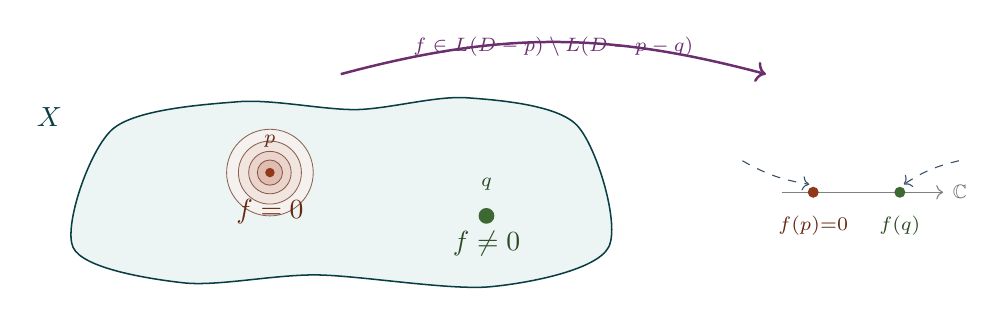
\begin{tikzpicture}[scale=1.0, every node/.style={font=\scriptsize}]
% Riemann surface silhouette
\filldraw[draw=formteal!55!black, fill=formteal!8, line width=0.55pt]
  plot[smooth cycle] coordinates {(-3.4,-0.7) (-2.9,0.8) (-1.3,1.15) (0.2,1.05) (1.6,1.2) (3.0,0.85) (3.4,-0.7) (1.9,-1.2) (-0.3,-1.05) (-2.0,-1.15)};
\node[formteal!55!black, font=\bfseries] at (-3.7,0.95) {$X$};
% Two distinguished points: p and q
\coordinate (P) at (-0.9,0.25);
\coordinate (Q) at (1.85,-0.3);
% At p: section vanishes (concentric fade-in)
\foreach \rr/\op in {0.55/8, 0.4/16, 0.27/26, 0.16/40}{
  \filldraw[draw=formrust!55!black, fill=formrust!\op, opacity=0.7, line width=0.3pt] (P) circle (\rr);
}
\fill[formrust!85!black] (P) circle (0.06);
\node[formrust!60!black, font=\scriptsize, above] at (-0.9,0.45) {$p$};
\node[formrust!60!black, font=\bfseries] at (-0.9,-0.25) {$f=0$};
% At q: section nonzero (filled dot, no vanishing rings)
\fill[formsage!85!black] (Q) circle (0.10);
\node[formsage!60!black, font=\scriptsize, above] at (1.85,-0.1) {$q$};
\node[formsage!60!black, font=\bfseries] at (1.85,-0.65) {$f\neq 0$};
% Arrow from X to C via f
\draw[->, formplum, line width=0.9pt] (0,1.5) to[bend left=15] (5.4,1.5);
\node[formplum, font=\scriptsize] at (2.7,1.85) {$f\in L(D-p)\setminus L(D-p-q)$};
% Target: complex line C, showing 0 and nonzero value
\begin{scope}[xshift=6.0cm]
  \draw[->, black!50, line width=0.4pt] (-0.4,0) -- (1.65,0) node[right, black!60] {$\C$};
  \fill[formrust!85!black] (0,0) circle (0.07);
  \node[formrust!60!black, font=\scriptsize, below] at (0,-0.18) {$f(p){=}0$};
  \fill[formsage!85!black] (1.1,0) circle (0.07);
  \node[formsage!60!black, font=\scriptsize, below] at (1.1,-0.18) {$f(q)$};
  \draw[->, formslate, line width=0.4pt, dashed] (-0.9,0.4) to[bend right=10] (-0.05,0.1);
  \draw[->, formslate, line width=0.4pt, dashed] (1.85,0.4) to[bend right=10] (1.15,0.1);
\end{scope}
\end{tikzpicture}
\visualcaption{When $\deg D\geq 2g+1$, the linear system $L(D)$ contains a section vanishing at $p$ but not at $q$. The two points are mapped to distinct values, so the sections of $L(D)$ separate points of $X$ — the first ingredient in showing the Kodaira map is an embedding.}
\end{center}

\section*{Problem 20: Separation of Tangent Directions and Immersions}

\begin{intentrequirements}
\item \textbf{Intent.} Prove that the same degree bound $\deg D\geq2g+1$ gives sections separating first-order tangent directions, so the associated Kodaira map is an immersion.
\item \textbf{Required outputs.} Produce $f_0,f_1\in L(D)$ with $f_0$ nonzero at $p$ and $f_1$ vanishing to exactly first order at $p$, then show the ratio $f_1/f_0$ has nonzero differential at $p$.
\item \textbf{Required explanations.} Use base point freeness for $f_0$, and compare $L(D-p)$ with $L(D-2p)$ to get a section with exact first-order vanishing.
\item \textbf{Common pitfalls to avoid.} It is not enough for a section to vanish at $p$; it must vanish to order exactly one. Order at least two would give zero tangent derivative.
\end{intentrequirements}

Assume
\[
 \deg D\geq2g+1.
\]
First, by Problem 18, $L(D)$ is base point free. Thus for every $p\in X$ there exists
\[
 f_0\in L(D)
\]
whose associated section is nonzero at $p$.

Next compare $D-p$ and $D-2p$. Their degrees satisfy
\[
 \deg(D-p)\geq2g,
\qquad
 \deg(D-2p)\geq2g-1.
\]
Asymptotic Riemann-Roch gives
\[
 \ell(D-p)=\deg D-g,
\]
and
\[
 \ell(D-2p)=\deg D-1-g.
\]
Therefore
\[
 \ell(D-p)-\ell(D-2p)=1.
\]
Choose
\[
 f_1\in L(D-p)\setminus L(D-2p).
\]
In a local trivialization, this says that $f_1$ vanishes at $p$ to order exactly $1$.

Thus $L(D)$ separates tangent directions: near $p$, the ratio
\[
 \frac{f_1}{f_0}
\]
is a local holomorphic function vanishing to first order. Therefore its differential at $p$ is nonzero. For the Kodaira map defined by a basis of $L(D)$, this implies
\[
 d\Phi_p\neq0.
\]
Hence the Kodaira map is an immersion at $p$. Since $p$ was arbitrary, it is an immersion everywhere.

In the notation of the problem, when ordinary function values are available in the chosen trivialization, this gives
\[
 f_0(p)\neq0,
\qquad
 \ord_p(f_1)=1.
\]

\section*{Problem 21: A Double Pole on a Complex Torus}

\begin{intentrequirements}
\item \textbf{Intent.} Use Riemann--Roch on a genus-one surface to produce a nonconstant meromorphic function with controlled pole order.
\item \textbf{Required outputs.} Apply Riemann--Roch to $D=2p$, prove $\ell(2p)=2$, conclude there is a nonconstant function with pole order at most $2$ at $p$, and show that if the torus is not $\CP^1$, the pole order must be exactly $2$.
\item \textbf{Required explanations.} Use that a complex torus has genus $1$ and trivial canonical degree. Thus $i(2p)=\ell(K-2p)=0$ because $\deg(K-2p)<0$.
\item \textbf{Common pitfalls to avoid.} A nonconstant function with a simple pole would define a degree-one map to $\CP^1$, forcing the torus to be biholomorphic to $\CP^1$.
\end{intentrequirements}

\windingnote{Why must the pole at $p$ have order exactly $2$ on a non-rational torus? A function with a simple pole at $p$ defines a degree-$1$ map $T\to\CP^1$ (the winding number of the function near $p$ is $1$), which by the sphere-characterization of Problem~17 would force $T\cong\CP^1$. The double pole, by contrast, gives a degree-$2$ map: locally near $p$, $f(z)\sim c/z^2$ and the winding number of $f$ around $\infty$ along a small loop is $2$. This is exactly the Weierstrass $\wp$-function, whose double pole is the natural generator of $L(2p)/\text{constants}$. The winding count distinguishes ``one wrap'' (sphere) from ``two wraps'' (torus).}

\handsketch{%
\fill[handpaper] (-3.4,-1.9) rectangle (3.4,1.9);
\draw[hand] (-3.4,-1.9) rectangle (3.4,1.9);
% Fundamental parallelogram of T
\draw[handthick] (-2.4,-1.1) -- (-0.8,-1.2) -- (0,0.95) -- (-1.6,1.1) -- cycle;
\foreach \xx in {-2.4,-2.0,-1.6,-1.2,-0.8}{
  \draw[draw=handink, line width=0.3pt, opacity=0.5]
    ($(\xx,-1.1)!\xx/2.4!(\xx,1.1)$) -- ++(0.8,2.05);
}
\node[handnote] at (-1.6,-1.45) {fund.\ parallelogram};
% Double pole at p
\fill[handink] (-1.2,0.0) circle (0.07);
\node[handnote] at (-1.25,-0.25) {$p$};
\draw[draw=handink, line width=0.55pt] (-1.2,0.0) circle (0.18);
\draw[draw=handink, line width=0.55pt] (-1.2,0.0) circle (0.32);
\node[handnote] at (-1.2,0.55) {order 2};
% Arrow to image
\draw[draw=handink, line width=0.8pt, -{Latex[length=2.5mm]}] (0.3,0) -- (1.4,0);
\node[handnote] at (0.85,0.3) {$\wp$};
% Image CP^1, winding 2
\begin{scope}[xshift=2.4cm]
  \draw[handthick] (0,0) circle (0.85);
  \draw[draw=handink, line width=0.55pt, smooth, samples=120, variable=\t, domain=0:720]
    plot ({(0.55+0.05*sin(4*\t))*cos(\t)},{(0.55+0.05*sin(4*\t))*sin(\t)});
  \fill[handink] (0,0) circle (0.04);
  \node[handnote] at (0.15,-0.18) {$\infty$};
  \node[handnote] at (0,-1.1) {winding 2};
\end{scope}
\node[handnote] at (0,1.5) {$\wp:T\to\CP^1$, degree 2};
}

Throughout Problem 21, let $T=\C/\Lambda$ be a complex torus and let $p\in T$. The genus of $T$ is $1$, and a canonical divisor has degree
\[
 2g-2=0.
\]
In fact, the form $dz$ descends to a nowhere-vanishing holomorphic $1$-form on $T$, so the canonical divisor is linearly equivalent to $0$.

\subsection*{Problem 21-1: Existence of a nonconstant $f\in\mathcal M(T)$ with pole of order at most $2$ at $p$}

Apply Riemann--Roch to $D=2p$. Since $\deg D=2$ and $g=1$,
\[
 \ell(2p)-i(2p)=\deg(2p)+1-g=2+1-1=2.
\]
By Problem 13,
\[
 i(2p)=\ell(K-2p),
\]
and the degree of $K-2p$ is
\[
 \deg(K-2p)=0-2=-2<0,
\]
so $\ell(K-2p)=0$, i.e.\ $i(2p)=0$. Therefore
\[
 \ell(2p)=2.
\]
Since constants form a one-dimensional subspace of $L(2p)$, the equality $\ell(2p)=2$ means there exists a nonconstant $f\in L(2p)$. By definition of $L(2p)$, such an $f$ has no poles except possibly at $p$, and the pole order at $p$ is at most $2$.

\subsection*{Problem 21-2: If $T\not\cong\CP^1$, the pole order at $p$ can be made exactly $2$}

Suppose $T$ is not biholomorphic to $\CP^1$. A nonconstant $f\in L(2p)$ must have a pole at $p$, because a holomorphic function on compact $T$ is constant. The pole order at $p$ is $1$ or $2$.

If every nonconstant $f\in L(2p)$ had a simple pole at $p$, then as a map
\[
 f:T\to\CP^1
\]
the fiber over $\infty$ would have total multiplicity $1$, so $\deg f=1$. A degree-one nonconstant holomorphic map between compact Riemann surfaces is biholomorphic, forcing $T\cong\CP^1$, a contradiction.

Therefore there exists a nonconstant $f\in L(2p)$ whose pole at $p$ has order exactly $2$.

\begin{center}
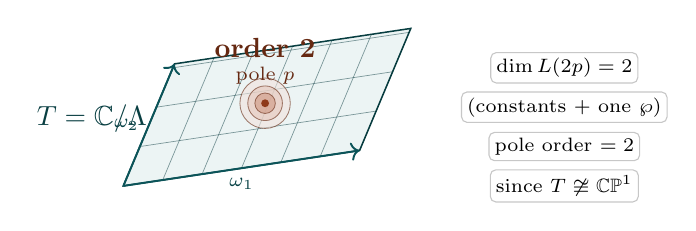
\begin{tikzpicture}[scale=1.0, every node/.style={font=\scriptsize}]
% Fundamental parallelogram
\filldraw[draw=formteal!55!black, fill=formteal!8, line width=0.55pt]
  (0,0) -- (3.0,0.45) -- (3.65,2.0) -- (0.65,1.55) -- cycle;
\foreach \xx in {0,0.5,...,3.0}{
  \draw[formteal!50!black, line width=0.25pt, opacity=0.5]
    ($(0,0)!\xx/3.0!(3.0,0.45)$) -- ($(0.65,1.55)!\xx/3.0!(3.65,2.0)$);
}
\foreach \yy in {0,0.5,...,1.55}{
  \draw[formteal!50!black, line width=0.25pt, opacity=0.5]
    ($(0,0)!\yy/1.55!(0.65,1.55)$) -- ($(3.0,0.45)!\yy/1.55!(3.65,2.0)$);
}
% Period vectors
\draw[->, formteal!75!black, line width=0.7pt] (0,0) -- (3.0,0.45) node[midway, below, formteal!60!black] {$\omega_1$};
\draw[->, formteal!75!black, line width=0.7pt] (0,0) -- (0.65,1.55) node[midway, left, formteal!60!black] {$\omega_2$};
% Double pole at p
\coordinate (P) at (1.8,1.05);
\foreach \rr/\op in {0.32/15, 0.22/30, 0.13/55}{
  \filldraw[draw=formrust!60!black, fill=formrust!\op, line width=0.3pt, opacity=0.6] (P) circle (\rr);
}
\fill[formrust!85!black] (P) circle (0.05);
\node[formrust!60!black, font=\scriptsize] at (1.8,1.4) {pole $p$};
\node[formrust!60!black, font=\bfseries] at (1.8,1.75) {order 2};
% Periods labels
\node[font=\scriptsize, fill=white, rounded corners=2pt, inner sep=2pt, draw=black!22]
  at (5.6,1.5) {$\dim L(2p)=2$};
\node[font=\scriptsize, fill=white, rounded corners=2pt, inner sep=2pt, draw=black!22]
  at (5.6,1.0) {(constants + one $\wp$)};
\node[font=\scriptsize, fill=white, rounded corners=2pt, inner sep=2pt, draw=black!22]
  at (5.6,0.5) {pole order $=2$};
\node[font=\scriptsize, fill=white, rounded corners=2pt, inner sep=2pt, draw=black!22]
  at (5.6,0.0) {since $T\not\cong\CP^1$};
\node[formteal!55!black, font=\bfseries] at (-0.4,0.85) {$T=\C/\Lambda$};
\end{tikzpicture}
\visualcaption{On the torus $T=\C/\Lambda$, Riemann--Roch forces $\dim L(2p)=2$. After subtracting constants, the remaining one-dimensional family must include a function with pole order exactly $2$ at $p$ — exactly the Weierstrass $\wp$-function up to constants.}
\end{center}

\section*{Problem 22: Minimal Polynomial of $\wp'$}

\begin{intentrequirements}
\item \textbf{Intent.} Derive the algebraic relation between $\wp$ and $\wp'$ and prove that it is the minimal polynomial of $\wp'$ over $\C(\wp)$.
\item \textbf{Required outputs.} Use the Laurent expansions of $\wp$ and $\wp'$ to choose constants $g_2,g_3$ such that
\[
 (\wp')^2=4\wp^3-g_2\wp-g_3,
\]
then prove the polynomial
\[
 T^2-(4\wp^3-g_2\wp-g_3)
\]
is minimal over $\C(\wp)$.
\item \textbf{Required explanations.} Show that the constructed elliptic function has removable poles and hence is constant on the compact torus. Then use parity: rational functions of even $\wp$ are even, while $\wp'$ is odd.
\item \textbf{Common pitfalls to avoid.} The quadratic relation alone proves algebraicity of degree at most two. Minimality requires the separate argument that $\wp'\notin\C(\wp)$.
\end{intentrequirements}

\windingnote{The Weierstrass functions $\wp,\wp'$ embed the torus $T=\C/\Lambda$ as the affine elliptic curve $y^2=4x^3-g_2x-g_3$. Each branch of this curve over a finite $x$-value contributes one sheet, and at the three roots of $4x^3-g_2x-g_3$ the two sheets meet at a ramification point of index $2$. The point at infinity is also a ramification point. Counting via the Riemann--Hurwitz residue form: the map $\wp:T\to\CP^1$ has degree $2$, four ramification points each with $e=2$, and $\chi(T)=0=2\cdot 2-\sum(2-1)=4-4$. The winding-form interpretation: at each branch point the local winding of $\wp$ is $2$, contributing $1$ to the ramification deficit; the total winding deficit equals $4=2\deg\wp$, balancing the topological identity. The minimal-polynomial relation $(y')^2=4y^3-g_2y-g_3$ is the algebraic shadow of this double-winding behavior.}

\handsketch{%
\fill[handpaper] (-3.4,-1.9) rectangle (3.4,1.9);
\draw[hand] (-3.4,-1.9) rectangle (3.4,1.9);
% Left: torus with 4 branch points
\begin{scope}[xshift=-1.85cm]
  \draw[handthick] (0,0) ellipse (1.0 and 0.55);
  \fill[white] (0,0) ellipse (0.4 and 0.16);
  \draw[draw=handink, line width=0.55pt] (0,0) ellipse (0.4 and 0.16);
  \foreach \xx in {-0.7,-0.1,0.5,1.0}{
    \fill[handink] (\xx,-0.55) circle (0.05);
  }
  \node[handnote] at (0,0.85) {$T^2$};
  \node[handnote] at (0,-1.0) {4 branch pts};
\end{scope}
% Map ℘
\draw[draw=handink, line width=0.8pt, -{Latex[length=2.5mm]}] (-0.7,0) -- (0.5,0);
\node[handnote] at (-0.1,0.3) {$\wp$};
% Right: elliptic curve y^2 = 4x^3 - g_2 x - g_3 (real locus)
\begin{scope}[xshift=2.0cm]
  \draw[draw=handink, line width=0.4pt] (-1.0,0) -- (1.4,0);
  \draw[draw=handink, line width=0.4pt] (0,-1.0) -- (0,1.1);
  \draw[draw=handink, line width=0.6pt, smooth, samples=60, variable=\x, domain=-0.8:0.2]
    plot (\x, {0.75*sqrt(max(0,(\x+0.8)*(0.2-\x)*(1.2-\x)))});
  \draw[draw=handink, line width=0.6pt, smooth, samples=60, variable=\x, domain=-0.8:0.2]
    plot (\x, {-0.75*sqrt(max(0,(\x+0.8)*(0.2-\x)*(1.2-\x)))});
  \draw[draw=handink, line width=0.6pt, smooth, samples=60, variable=\x, domain=1.2:1.4]
    plot (\x, {0.75*sqrt(max(0,(\x+0.8)*(\x-0.2)*(\x-1.2)))});
  \draw[draw=handink, line width=0.6pt, smooth, samples=60, variable=\x, domain=1.2:1.4]
    plot (\x, {-0.75*sqrt(max(0,(\x+0.8)*(\x-0.2)*(\x-1.2)))});
  \foreach \xx in {-0.8,0.2,1.2}{
    \fill[handink] (\xx,0) circle (0.05);
  }
  \node[handnote] at (0.3,1.2) {$y^2=4x^{3}-g_{2}x-g_{3}$};
\end{scope}
\node[handnote] at (0,-1.85) {ramification index 2 at each root + $\infty$};
}

Throughout Problem 22, let $\wp$ be the Weierstrass function for a lattice $\Lambda$, with Laurent expansion
\[
 \wp(z)=\frac1{z^2}+a_2z^2+a_4z^4+O(z^6).
\]
Differentiating term-by-term,
\[
 \wp'(z)=-\frac2{z^3}+2a_2z+4a_4z^3+O(z^5).
\]

\subsection*{Problem 22-1: Show $(\wp')^2=4\wp^3-g_2\wp-g_3$ for suitable $g_2,g_3$}

Compute the principal parts at $z=0$. Squaring the Laurent series for $\wp'$,
\[
(\wp')^2
=
4z^{-6}-8a_2z^{-2}-16a_4+O(z^2),
\]
and cubing the Laurent series for $\wp$,
\[
4\wp^3
=
4z^{-6}+12a_2z^{-2}+12a_4+O(z^2).
\]
Subtracting,
\[
(\wp')^2-4\wp^3
=
-20a_2z^{-2}-28a_4+O(z^2).
\]
Choose constants
\[
 g_2=20a_2,\qquad g_3=28a_4,
\]
and set
\[
 F(z)=(\wp')^2-4\wp^3+g_2\wp+g_3.
\]
By the choice of $g_2,g_3$, the principal-part contributions $-20a_2z^{-2}-28a_4$ are cancelled by $g_2\wp+g_3=20a_2\cdot z^{-2}+28a_4+O(z^2)$. So $F$ has no pole at $0$.

Since $\wp$ and $\wp'$ are elliptic, $F$ is elliptic. Its only possible poles modulo $\Lambda$ are at the lattice points, and the above calculation shows those poles are removable. Hence $F$ is a holomorphic function on the compact torus $\C/\Lambda$, so by maximum modulus (or Liouville on the universal cover) $F$ is constant. The Laurent expansion further shows that the constant term of $F$ is $0$, so
\[
 F\equiv0,
\]
which gives
\[
 \boxed{(\wp')^2=4\wp^3-g_2\wp-g_3.}
\]

\subsection*{Problem 22-2: Deduce the minimal polynomial of $\wp'$ over $\C(\wp)$}

The relation from 22-1 says that the polynomial
\[
 P(T)=T^2-\bigl(4\wp^3-g_2\wp-g_3\bigr)\in\C(\wp)[T]
\]
annihilates $\wp'$. Hence $\wp'$ is algebraic over $\C(\wp)$ of degree at most $2$.

It remains to show that $P(T)$ is minimal, i.e.\ that $\wp'\notin\C(\wp)$. Suppose toward a contradiction that
\[
 \wp'(z)=R(\wp(z))
\]
for some rational function $R$. Recall that $\wp$ is even and $\wp'$ is odd:
\[
 \wp(-z)=\wp(z),\qquad \wp'(-z)=-\wp'(z).
\]
Therefore any rational function of $\wp$ is even, so $R(\wp(z))=R(\wp(-z))$, contradicting $\wp'(-z)=-\wp'(z)\neq\wp'(z)$ for a nonzero $\wp'$. Hence $\wp'\notin\C(\wp)$, so $P(T)$ has degree exactly $2$ and is the minimal polynomial:
\[
 \boxed{T^2-\bigl(4\wp^3-g_2\wp-g_3\bigr).}
\]

\begin{center}
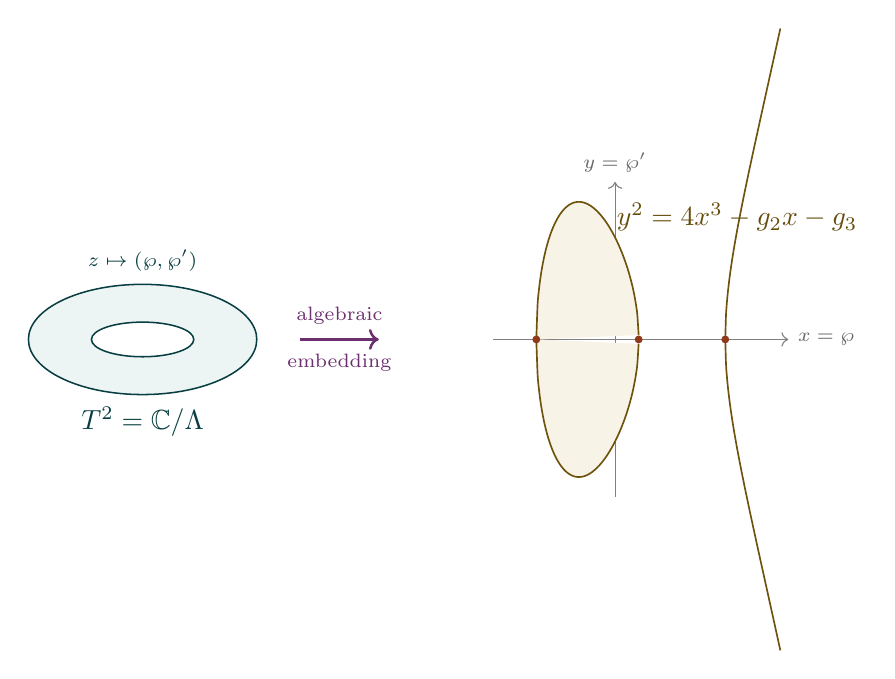
\begin{tikzpicture}[scale=1.0, every node/.style={font=\scriptsize}]
% Left: torus
\begin{scope}
  \filldraw[draw=formteal!55!black, fill=formteal!8, line width=0.55pt]
    (0,0) ellipse (1.45 and 0.7);
  \fill[white] (0,0) ellipse (0.65 and 0.22);
  \draw[formteal!55!black, line width=0.55pt] (0,0) ellipse (0.65 and 0.22);
  \node[formteal!55!black, font=\bfseries] at (0,-1.05) {$T^2=\C/\Lambda$};
  \node[formteal!55!black, font=\scriptsize] at (0,1.0) {$z\mapsto(\wp,\wp')$};
\end{scope}
% Arrow
\draw[->, formplum, line width=0.9pt] (2.0,0) -- (3.0,0);
\node[formplum, font=\scriptsize] at (2.5,0.3) {algebraic};
\node[formplum, font=\scriptsize] at (2.5,-0.3) {embedding};
% Right: elliptic curve y^2 = 4x^3 - g_2 x - g_3
\begin{scope}[xshift=6.0cm]
  \draw[->, black!50, line width=0.4pt] (-1.55,0) -- (2.2,0) node[right, black!60] {$x=\wp$};
  \draw[->, black!50, line width=0.4pt] (0,-2.0) -- (0,2.0) node[above, black!60] {$y=\wp'$};
  % Elliptic curve y^2 = (x-a)(x-b)(x-c) for some real a,b,c
  % Use a=-1, b=0.3, c=1.4 for a real curve. So y = sqrt(4(x-(-1))(x-0.3)(x-1.4)).
  % Plot two branches via parametric
  \draw[draw=formgold!60!black, fill=formgold!10, line width=0.6pt, smooth, samples=80, variable=\x, domain=-1:0.3]
    plot ({\x},{sqrt(max(0,4*(\x+1)*(0.3-\x)*(1.4-\x)))});
  \draw[draw=formgold!60!black, fill=formgold!10, line width=0.6pt, smooth, samples=80, variable=\x, domain=-1:0.3]
    plot ({\x},{-sqrt(max(0,4*(\x+1)*(0.3-\x)*(1.4-\x)))});
  \draw[draw=formgold!60!black, line width=0.6pt, smooth, samples=80, variable=\x, domain=1.4:2.1]
    plot ({\x},{sqrt(max(0,4*(\x+1)*(\x-0.3)*(\x-1.4)))});
  \draw[draw=formgold!60!black, line width=0.6pt, smooth, samples=80, variable=\x, domain=1.4:2.1]
    plot ({\x},{-sqrt(max(0,4*(\x+1)*(\x-0.3)*(\x-1.4)))});
  % Roots
  \foreach \rt in {-1,0.3,1.4}{
    \fill[formrust!85!black] (\rt,0) circle (0.05);
  }
  \node[formgold!55!black, font=\bfseries] at (1.55,1.55) {$y^2=4x^3-g_2x-g_3$};
\end{scope}
\end{tikzpicture}
\visualcaption{The Weierstrass map $(\wp,\wp'):T\to\C^2$ embeds the complex torus as the affine cubic curve $y^2=4x^3-g_2x-g_3$. The two branches over $x$ come from $\wp(z)$ and $\wp(-z)=\wp(z)$ having opposite $\wp'$-values, exactly the parity argument behind $\wp'\notin\C(\wp)$.}
\end{center}

\section*{Additional Extremely Detailed Notes, Keyed by Problem Number}

This section expands the main solutions above. It is intentionally redundant: the goal is to make clear which theorem is being used, why each hypothesis matters, and how the local-coordinate computations work.

\subsection*{Extra detail for Problem 1}

The Identity Theorem is really a theorem about isolated zeros. The key local fact is:
if $h$ is holomorphic near $a$ and $h$ is not identically zero near $a$, then the zeros of $h$ near $a$ are isolated.

Here is the local argument in slow motion. A holomorphic function has a Taylor expansion
\[
 h(z)=c_0+c_1(z-a)+c_2(z-a)^2+\cdots.
\]
If all coefficients are zero, then $h$ is zero on a disk around $a$. If not, choose the first nonzero coefficient $c_m$. Then
\[
 h(z)=(z-a)^m(c_m+c_{m+1}(z-a)+\cdots).
\]
The factor in parentheses is nonzero at $a$, so it remains nonzero on some small disk. Therefore, inside that small disk, the only zero is $z=a$. That is what it means for $a$ to be an isolated zero.

Connectedness enters only at the end. Once $h$ vanishes on one small open disk, analytic continuation by overlapping disks forces it to vanish throughout the whole connected domain. Without connectedness, a holomorphic function could vanish on one component and not on another.

\subsection*{Extra detail for Problem 2}

There are two functions:
\[
 f(z)=\sin z
\]
and
\[
 g(z)=\sum_{n=0}^{\infty}(-1)^n\frac{z^{2n+1}}{(2n+1)!}.
\]
The power series has infinite radius of convergence because the factorial grows faster than every power of $z$. Thus $g$ is entire.

The real Maclaurin theorem says that for every real $x$,
\[
 \sin x=x-\frac{x^3}{3!}+\frac{x^5}{5!}-\cdots.
\]
So $f$ and $g$ agree on the real line. The real line is not open in $\C$, but that is not required. The Identity Theorem only requires an infinite set of agreement points having an accumulation point inside the domain. The set $\R\subset\C$ has accumulation point $0\in\C$. Therefore $f-g$ is an entire function whose zeros accumulate at $0$, and so $f-g\equiv0$.

The conceptual point is that a holomorphic function is determined globally on a connected domain by its values on a very small set, provided that set has a limit point in the domain.

\subsection*{Extra detail for Problem 3}

The Open Mapping Theorem says that nonconstant holomorphic functions cannot collapse open sets into curves or thin sets. The proof uses the local form of a holomorphic function near a zero.

If $f(a)=w_0$, then the function
\[
 f(z)-w_0
\]
has a zero at $a$. If $f$ is not locally constant, this zero has a finite order $m$. Therefore
\[
 f(z)-w_0=(z-a)^m u(z),
\]
where $u(a)\neq0$. This local form means that, near $a$, the map looks like
\[
 z\mapsto z^m
\]
up to nonvanishing holomorphic factors and coordinate changes. The map $z\mapsto z^m$ sends small disks onto small disks, though with multiplicity $m$.

The Rouche argument makes this precise. On a small circle $|z-a|=r$, the quantity $|f(z)-w_0|$ has a positive minimum because the circle is compact and there are no zeros on the circle. If $w$ is close enough to $w_0$, then $f(z)-w$ has the same number of zeros inside the circle as $f(z)-w_0$. Hence some $z$ near $a$ satisfies $f(z)=w$.

Thus every point $w_0=f(a)$ is an interior point of the image.

\subsection*{Extra detail for Problem 4}

The disk
\[
 B_1(1)=\{z:|z-1|<1\}
\]
is tangent to the origin but does not contain the origin. This matters because
\[
 f'(z)=2z
\]
vanishes only at $z=0$. Since $0$ lies on the boundary and not inside the disk, $f$ has nonzero derivative at every point of $B_1(1)$.

Therefore $f(z)=z^2$ is locally invertible throughout the disk. Local invertibility immediately implies local openness. Globally the image might overlap itself, but openness is local: every image point has a small open neighborhood contained in the image.

The Open Mapping Theorem gives the conclusion even faster, because $z^2$ is holomorphic and nonconstant on the open connected disk.

\subsection*{Extra detail for Problem 5}

The proposition is the compact Riemann surface version of the idea that a nonconstant holomorphic map behaves like a finite-sheeted covering, except at finitely many ramification points.

The local model is essential. If $x\in X$ and $f(x)=y$, choose coordinates $z$ near $x$ and $w$ near $y$ with $z(x)=0$ and $w(y)=0$. Then
\[
 w\circ f(z)=a_ez^e+a_{e+1}z^{e+1}+\cdots,\qquad a_e\neq0.
\]
After a holomorphic coordinate change in the target, this becomes
\[
 w=z^e.
\]
The integer $e=e_x(f)$ is the ramification index. If $e=1$, the map is locally biholomorphic. If $e>1$, the point is ramified.

Surjectivity uses compactness and openness:
\[
 f(X)\text{ compact}\Rightarrow f(X)\text{ closed},
\]
and the Open Mapping Theorem gives
\[
 f(X)\text{ open}.
\]
Since $Y$ is connected, the image is all of $Y$.

Finiteness of fibers uses the Identity Theorem. If infinitely many points in a fiber accumulated, then the local equation $f-y=0$ would have accumulating zeros, forcing $f$ to be locally constant.

The degree formula
\[
 \sum_{x\in f^{-1}(y)}e_x(f)=\deg f
\]
means that ramified points count multiple times. In the model $w=z^e$, a nearby nonzero value of $w$ has exactly $e$ preimages near $z=0$.

\subsection*{Extra detail for Problem 6}

For a nonconstant map
\[
 f:T^2\to\CP^1,
\]
Problem 5 says $f$ is a branched covering. Away from finitely many branch values, every point of $\CP^1$ has exactly $\deg f$ preimages. Over a branch value, some of these preimages collide, and the ramification index records the collision multiplicity.

Riemann-Hurwitz gives
\[
 \chi(T^2)=(\deg f)\chi(\CP^1)-\sum_{x\in T^2}(e_x-1).
\]
Since
\[
 \chi(T^2)=0,\qquad \chi(\CP^1)=2,
\]
we get
\[
 \sum_{x\in T^2}(e_x-1)=2\deg f.
\]
So a nonconstant holomorphic map from a torus to the sphere must ramify. There is no unramified covering $T^2\to\CP^1$ because an unramified degree-$n$ cover would force
\[
 0=n\cdot2,
\]
which is impossible.

\subsection*{Extra detail for Problem 7}

A polynomial $p(z)$ of degree $n$ becomes a holomorphic map
\[
 P:\CP^1\to\CP^1.
\]
The only point that needs checking is $\infty$. Use $w=1/z$ near $\infty$ in the source and $\zeta=1/u$ near $\infty$ in the target. If
\[
 p(z)=a_nz^n+a_{n-1}z^{n-1}+\cdots,
\]
then
\[
 p(1/w)=a_nw^{-n}+a_{n-1}w^{-(n-1)}+\cdots.
\]
Thus
\[
 \frac{1}{p(1/w)}
 =
 \frac{w^n}{a_n+a_{n-1}w+\cdots},
\]
which is holomorphic at $w=0$ and vanishes there. This proves that $P(\infty)=\infty$ holomorphically.

Now compactness enters. A nonconstant holomorphic map between compact connected Riemann surfaces is surjective. Hence $0$ lies in the image of $P$. Since $P(\infty)=\infty$, the preimage of $0$ must be a finite complex number $z_0$. Therefore $p(z_0)=0$.

\subsection*{Extra detail for Problem 8}

The residue of a meromorphic $1$-form is coordinate independent because it is detected by an integral:
\[
 \Res_p(\omega)=\frac{1}{2\pi i}\int_{\gamma}\omega
\]
where $\gamma$ is a small positively oriented loop around $p$. Integrals of differential forms are intrinsic. Changing coordinates only changes the way the same loop and same form are written.

For the residue sum, remove small disks around all poles:
\[
 M^\circ=M\setminus\bigcup_j B_j.
\]
The boundary of $M^\circ$ is a union of negatively oriented circles around the removed disks. This is the most common sign mistake in this problem. The orientation is negative because when walking along the boundary of the remaining surface, the surface must stay on the left; around a hole that forces clockwise motion.

On $M^\circ$, the form is holomorphic, so in local coordinates $\omega=f(z)dz$ with $f$ holomorphic. Then
\[
 d\omega=df\wedge dz=f'(z)dz\wedge dz=0.
\]
Stokes gives
\[
 0=\int_{M^\circ}d\omega=\int_{\partial M^\circ}\omega
 =-\sum_j\int_{\partial B_j}\omega.
\]
Each positively oriented disk boundary integral is $2\pi i$ times the residue, giving
\[
 \sum_j\Res_{p_j}(\omega)=0.
\]

\subsection*{Extra detail for Problem 9}

The logarithmic derivative
\[
 \frac{df}{f}
\]
turns orders of zeros and poles into residues.

If $f$ has order $m$ at $p$, then locally
\[
 f=z^m u(z),
\]
where $u(0)\neq0$. This notation handles zeros and poles at once:
\[
 m>0 \text{ for a zero},\qquad m<0 \text{ for a pole}.
\]
Then
\[
 df=mz^{m-1}u(z)dz+z^m u'(z)dz,
\]
so
\[
 \frac{df}{f}
 =
 m\frac{dz}{z}+\frac{u'(z)}{u(z)}dz.
\]
The second term is holomorphic. Hence the only residue is $m$.

The residue theorem then says
\[
 0=\sum_p\Res_p(df/f)=\sum_p\ord_p(f).
\]
That is exactly
\[
 \deg(f)=0.
\]
So the number of zeros equals the number of poles, counted with multiplicity, on a compact Riemann surface.

\subsection*{Extra detail for Problem 10}

For
\[
 f(z)=\frac{z^2(z-1)}{(z-2)^3},
\]
finite zeros and poles are read directly:
\[
 0\text{ is a zero of order }2,\quad
 1\text{ is a zero of order }1,\quad
 2\text{ is a pole of order }3.
\]
The only subtle point is infinity. Use $w=1/z$. Then
\[
 f(1/w)=\frac{w^{-2}(w^{-1}-1)}{(w^{-1}-2)^3}
 =
 \frac{1-w}{(1-2w)^3}.
\]
At $w=0$, this equals $1$, so there is neither a zero nor a pole at infinity.

For $dz$, the affine coordinate hides the pole at infinity. Since
\[
 z=\frac1w,
\]
we have
\[
 dz=-\frac{1}{w^2}dw.
\]
Thus $dz$ has a double pole at infinity and no finite zeros or poles. Therefore
\[
 (dz)=-2[\infty].
\]
This is the canonical divisor on $\CP^1$, whose degree is $-2=2g-2$ for $g=0$.

\subsection*{Extra detail for Problem 11}

Riemann-Hurwitz is Euler characteristic bookkeeping.

The cleanest proof is by triangulation. Put every branch value of $f:X\to Y$ among the vertices of a triangulation of $Y$. Then pull the triangulation back to $X$.

Faces and edges do not contain branch values in their interiors, so each face and edge lifts to exactly $n=\deg f$ copies:
\[
 F_X=nF_Y,\qquad E_X=nE_Y.
\]
Vertices are different. If $y$ is a vertex, then the number of vertices above $y$ is not necessarily $n$. Instead,
\[
 \sum_{x\in f^{-1}(y)}e_x=n.
\]
Therefore
\[
 \#f^{-1}(y)=n-\sum_{x\in f^{-1}(y)}(e_x-1).
\]
Summing over all vertices gives the correction term. Substituting into
\[
 \chi=V-E+F
\]
gives
\[
 \chi(X)=n\chi(Y)-\sum_x(e_x-1).
\]

\subsection*{Extra detail for Problem 12}

The statement
\[
 \deg K=2g-2
\]
is equivalent to
\[
 \deg(\omega)=-\chi(M)
\]
because $\chi(M)=2-2g$.

The proof using Riemann-Hurwitz compares a meromorphic differential to the differential of a meromorphic function. If
\[
 f:M\to\CP^1
\]
has degree $n$, then Riemann-Hurwitz says
\[
 \chi(M)=2n-\sum_p(e_p-1).
\]
The divisor of $df$ has two kinds of contributions:
\begin{itemize}
\item At points where $f$ is finite, local form $f(z)=z^e$ gives $df=ez^{e-1}dz$, so contribution $e-1$.
\item At points over infinity, local form $f(z)=z^{-e}$ gives $df=-ez^{-e-1}dz$, so contribution $-(e+1)=(e-1)-2e$.
\end{itemize}
Summing over all points gives
\[
 \deg(df)=\sum_p(e_p-1)-2\deg f.
\]
By Riemann-Hurwitz this is
\[
 -\chi(M).
\]
Any other meromorphic $1$-form differs from $df$ by multiplication by a meromorphic function, whose divisor has degree zero. Hence all canonical divisors have the same degree.

\subsection*{Extra detail for Problem 13}

Fix a meromorphic $1$-form $\eta$ with divisor $K$. Multiplying a meromorphic function by $\eta$ converts function divisors into differential divisors:
\[
 (f\eta)=(f)+(\eta)=(f)+K.
\]

For $I(K-D)\cong L(D)$, check the defining inequality:
\[
 f\in L(D)
 \Longleftrightarrow
 (f)+D\geq0.
\]
On the other hand,
\[
 f\eta\in I(K-D)
 \Longleftrightarrow
 (f\eta)-(K-D)\geq0.
\]
Substitute $(f\eta)=(f)+K$:
\[
 (f)+K-K+D=(f)+D\geq0.
\]
So the conditions are identical.

The proof of $\ell(p)\leq2$ has two cases. If all functions in $L(p)$ are constant, then $\ell(p)=1$. If a nonconstant function exists with at most a simple pole at $p$, it defines a degree-one map to $\CP^1$. Degree one forces a biholomorphism. Then $X\cong\CP^1$, and $L(p)$ has basis $\{1,z\}$ after sending $p$ to infinity.

\subsection*{Extra detail for Problem 14}

The principal-parts criterion is a global residue obstruction. A meromorphic function with prescribed principal parts exists exactly when multiplying those principal parts by any holomorphic differential gives total residue zero.

For effective
\[
 D=\sum m_j a_j,
\]
the allowed principal part at $a_j$ has $m_j$ coefficients:
\[
 c_{j,1}z^{-1}+c_{j,2}z^{-2}+\cdots+c_{j,m_j}z^{-m_j}.
\]
Thus the total space of possible principal parts has dimension
\[
 \sum_jm_j=\deg D.
\]

The map from $L(D)$ to principal parts has kernel equal to the holomorphic functions. On compact $X$, those are constants. Hence image dimension is $\ell(D)-1$.

The obstruction map lands in the dual of the $g$-dimensional space of holomorphic $1$-forms. Its rank is $g-i(D)$ because the holomorphic differentials annihilating every allowed principal part are exactly those with enough zeros to lie in $I(D)$.

Therefore
\[
 \ell(D)-1=\deg D-(g-i(D)),
\]
which rearranges to Riemann-Roch for effective divisors:
\[
 \ell(D)-i(D)=\deg D+1-g.
\]

\subsection*{Extra detail for Problem 15}

The goal is to extend Riemann-Roch from effective divisors to arbitrary divisors by subtracting one point at a time.

The inclusions are
\[
 L(D-a)\subset L(D),
\]
because allowing divisor $D$ permits one more order of pole at $a$ than allowing $D-a$.
The quotient has dimension at most one because only one Laurent coefficient at $a$ is newly allowed.

For differentials,
\[
 I(D)\subset I(D-a),
\]
because the condition $(\omega)-D\geq0$ is stricter than $(\omega)-(D-a)\geq0$.
Again the dimension can increase by at most one.

The key contradiction prevents both jumps from happening simultaneously. If both jumps occurred, there would be a function $f$ and a differential $\omega$ such that $f\omega$ has a single simple pole at $a$ with nonzero residue and no other poles. This violates the residue theorem. Hence the error term in Riemann-Roch cannot decrease while subtracting points. Starting from an effective divisor proves the inequality for all divisors.

\subsection*{Extra detail for Problem 16}

Problem 15 gives
\[
 \ell(E)-i(E)\geq\deg E+1-g
\]
for every divisor $E$. Put
\[
 E=K-D.
\]
Then
\[
 \ell(K-D)-i(K-D)\geq \deg K-\deg D+1-g.
\]
Using
\[
 \ell(K-D)=i(D),\qquad i(K-D)=\ell(D),
\]
we get
\[
 i(D)-\ell(D)\geq \deg K-\deg D+1-g.
\]
This is the reverse inequality after multiplying by $-1$ and substituting
\[
 \deg K=2g-2.
\]
Combining with Problem 15 gives equality. This is a common structure in Riemann-Roch proofs: one inequality is direct, and the other is obtained by duality with $K-D$.

\subsection*{Extra detail for Problem 17}

The equivalence connects three ways to recognize genus zero:
\[
 \text{topological sphere}
 \Longleftrightarrow
 \text{existence of a function with one simple pole}
 \Longleftrightarrow
 \text{Riemann sphere}.
\]

If $\ell(p)\geq2$, then there is a nonconstant function in $L(p)$. Such a function has at most one simple pole. It must have a pole, because a holomorphic function on compact $X$ is constant. Thus it has exactly one simple pole. The map to $\CP^1$ has degree equal to the total pole order, namely $1$. A degree-one holomorphic map is a biholomorphism.

Conversely, if $X$ is topologically $S^2$, then $g=0$. Riemann-Roch gives
\[
 \ell(p)-i(p)=2.
\]
The term $i(p)$ vanishes because it would require a meromorphic differential with divisor degree at least $1$, but every canonical divisor has degree $-2$ on genus zero. Hence $\ell(p)=2$.

\subsection*{Extra detail for Problem 18}

Asymptotic Riemann-Roch says that when $\deg D$ is large enough, the correction term disappears:
\[
 i(D)=\ell(K-D)=0
\]
because
\[
 \deg(K-D)=2g-2-\deg D<0.
\]
A divisor of negative degree cannot be the divisor of a nonzero meromorphic function plus an effective divisor condition, so $L(K-D)=0$.

Base point freeness is best stated intrinsically for the line bundle $\mathcal O(D)$. The point $p$ is not a base point if there is a section not vanishing at $p$. In divisor notation this is equivalent to
\[
 L(D-p)\subsetneq L(D).
\]
When $\deg D\geq2g$, both $D$ and $D-p$ are in the asymptotic range. Riemann-Roch gives
\[
 \ell(D)-\ell(D-p)=1.
\]
Therefore the inclusion is strict, so a section exists that does not vanish at $p$.

\subsection*{Extra detail for Problem 19}

To separate two points $p\neq q$, it is enough to find a section vanishing at one but not the other. Intrinsically, this means
\[
 L(D-p)\neq L(D-p-q).
\]
If
\[
 \deg D\geq2g+1,
\]
then
\[
 \deg(D-p)\geq2g,\qquad \deg(D-p-q)\geq2g-1.
\]
Both are greater than $2g-2$, so asymptotic Riemann-Roch applies to both. The dimensions differ by one:
\[
 \ell(D-p)-\ell(D-p-q)=1.
\]
Hence there is a section in $L(D-p)$ not in $L(D-p-q)$. It vanishes at $p$ but not at $q$, so it separates the points.

\subsection*{Extra detail for Problem 20}

Separating tangent directions means producing a local coordinate from ratios of sections. At a point $p$, choose
\[
 f_0\in L(D)
\]
nonzero at $p$ using base point freeness. Then compare $D-p$ and $D-2p$. Asymptotic Riemann-Roch gives
\[
 \ell(D-p)-\ell(D-2p)=1.
\]
So there is
\[
 f_1\in L(D-p)\setminus L(D-2p).
\]
Locally this means $f_1$ vanishes to exactly first order at $p$.

The ratio
\[
 \frac{f_1}{f_0}
\]
is then a holomorphic function near $p$ with a simple zero. Its differential is nonzero at $p$. Since this ratio is one affine coordinate of the Kodaira map, the differential of the Kodaira map is nonzero. Therefore the Kodaira map is an immersion.

\subsection*{Extra detail for Problem 21}

For a complex torus, $g=1$. Riemann-Roch for $D=2p$ says
\[
 \ell(2p)-i(2p)=2+1-1=2.
\]
The correction term is
\[
 i(2p)=\ell(K-2p).
\]
On a torus, $K$ has degree $0$, so $K-2p$ has degree $-2$. A divisor of negative degree has no nonzero functions in its $L$-space, so $i(2p)=0$. Hence
\[
 \ell(2p)=2.
\]
Since constants account for only one dimension, there is a nonconstant meromorphic function with pole of order at most $2$ at $p$ and no other poles.

If the pole order were $1$, the function would define a degree-one map to $\CP^1$. That would make the torus biholomorphic to $\CP^1$. Since this is excluded, the pole order must be exactly $2$.

\subsection*{Extra detail for Problem 22}

The Weierstrass function $\wp$ is even, elliptic, and has a double pole at each lattice point. Its derivative $\wp'$ is odd, elliptic, and has a triple pole at each lattice point.

The strategy is to build an elliptic function with no poles:
\[
 F=(\wp')^2-4\wp^3+g_2\wp+g_3.
\]
The constants $g_2,g_3$ are chosen to cancel the principal part at the lattice points. Because the function is elliptic, it is enough to check one lattice point, say $0$.

Using
\[
 \wp=z^{-2}+a_2z^2+a_4z^4+O(z^6)
\]
and
\[
 \wp'=-2z^{-3}+2a_2z+4a_4z^3+O(z^5),
\]
we get
\[
(\wp')^2-4\wp^3=-20a_2z^{-2}-28a_4+O(z^2).
\]
Choosing
\[
 g_2=20a_2,\qquad g_3=28a_4
\]
cancels the pole and constant term. Thus $F$ is holomorphic on the compact torus, so it is constant; the expansion shows the constant is zero.

The minimal polynomial has degree two because $\wp'$ satisfies a quadratic equation over $\C(\wp)$, but $\wp'$ is not itself in $\C(\wp)$. The parity argument proves this: every rational function of the even function $\wp$ is even, while $\wp'$ is odd and nonzero.

\end{document}
